\begin{appendices}

\chapter{Cut and Match Results}
\label{App:CutAndMatchingResults}

\newpage 

\section{Cut Results}
\label{sec:CutResults}

\begin{figure}[H]
  \centering
  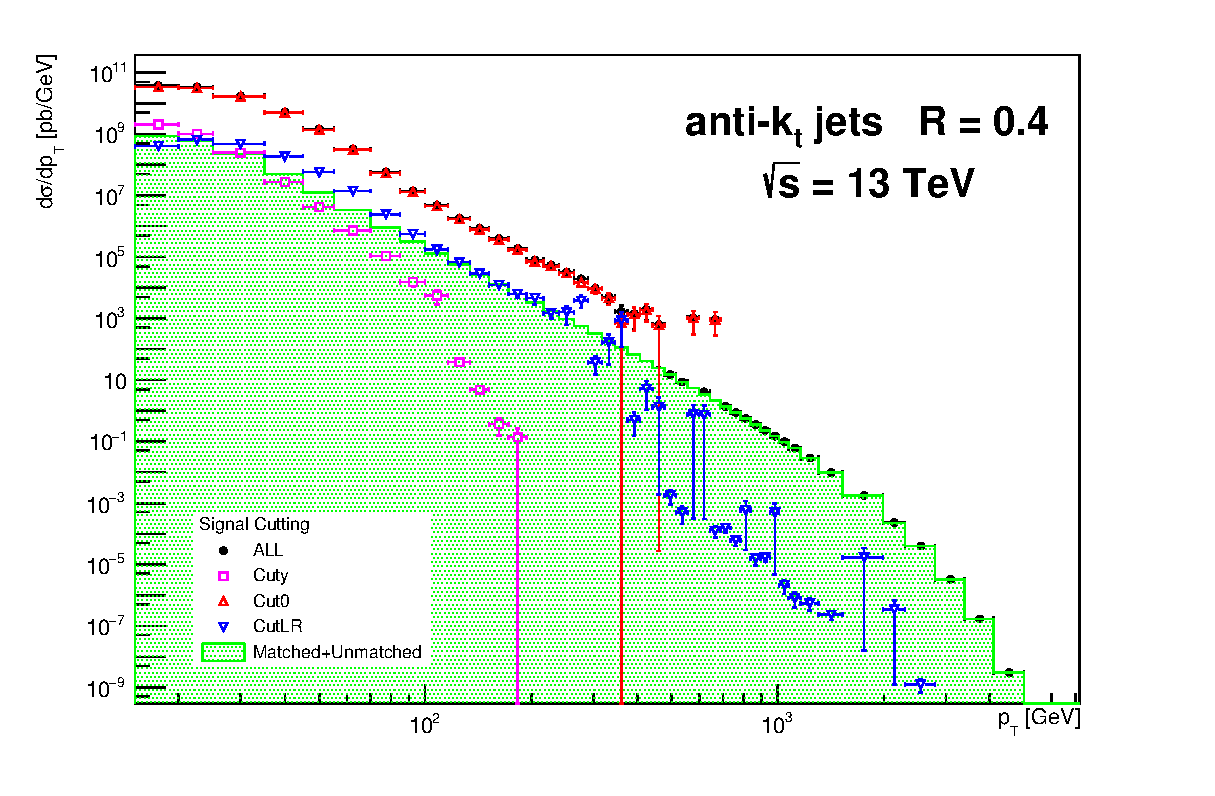
\includegraphics[width=\textwidth]{Chapter3/SignalCutting.eps}
  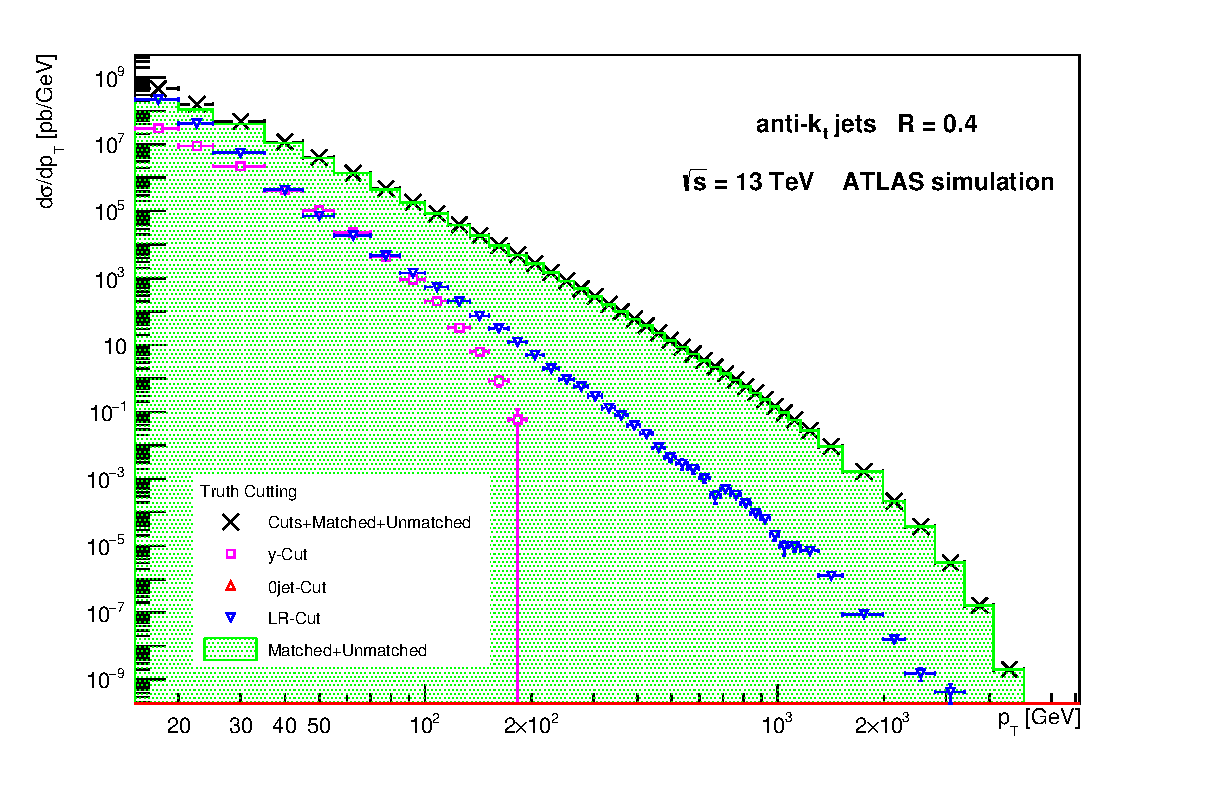
\includegraphics[width=\textwidth]{Chapter3/TruthCutting.eps}
  \caption{Impact of 4 cuts defined in Section \ref{SubSec:JetCuts} on
  differential cross section in $\pt$ of reco jets (top) and truth jets
  (bottom). Black dots represent the original uncutted spectrum, green area then
  these jets, which survived all four cutoffs.}
  \label{fig:Cutting}
\end{figure}

\section{Match Results}
\label{sec:MatchResults}

\begin{figure}[H]
  \centering
  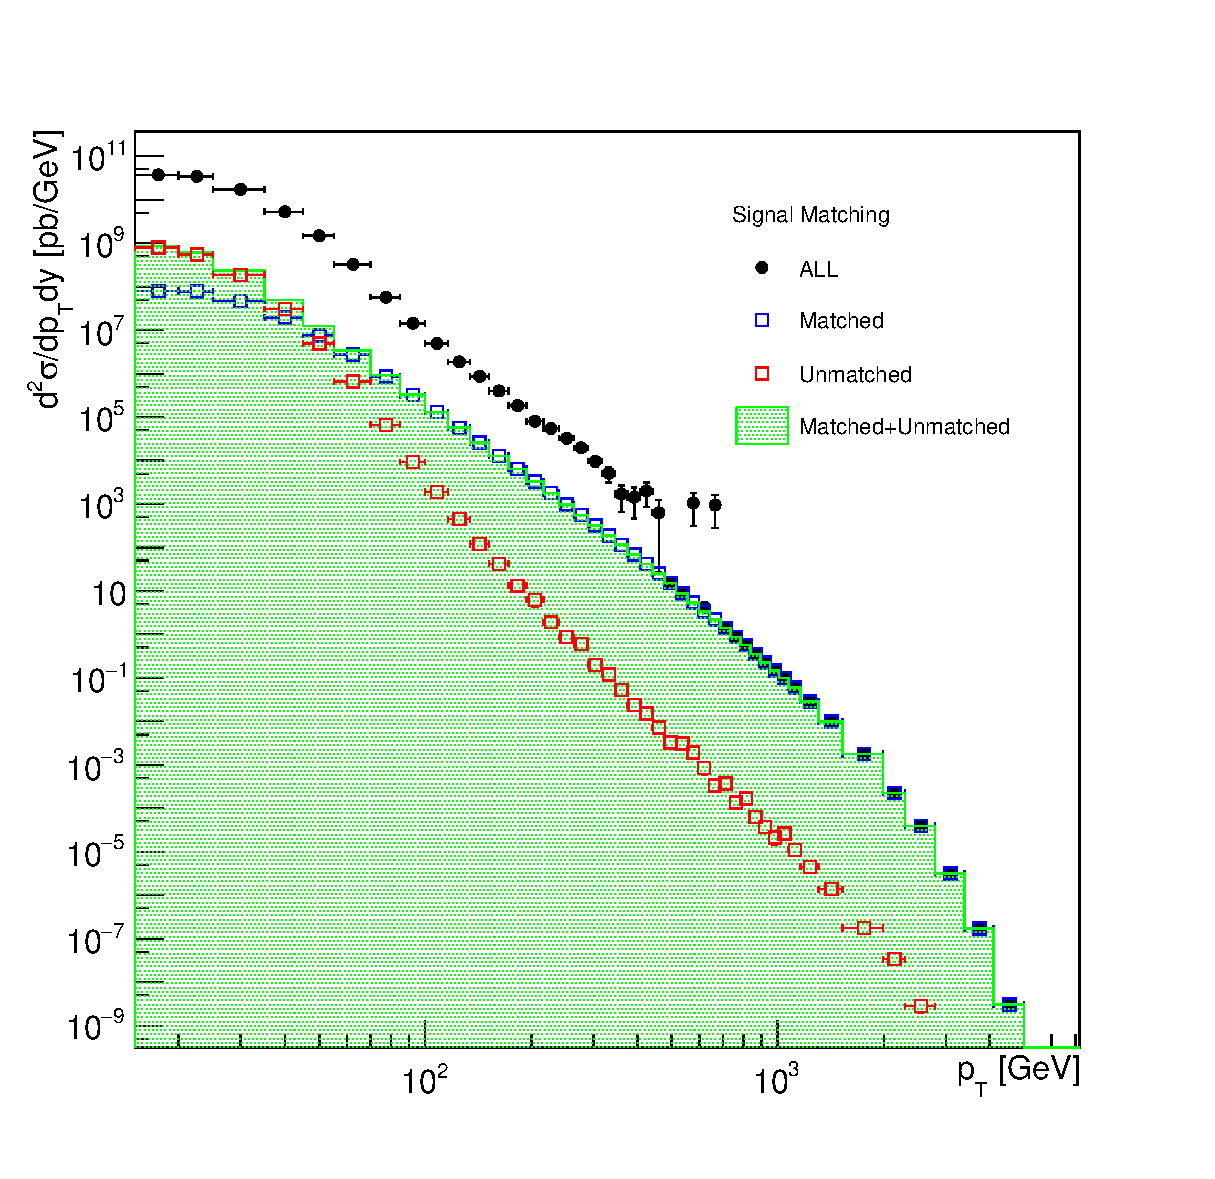
\includegraphics[width=\textwidth]{Chapter3/SignalMatching.eps}
  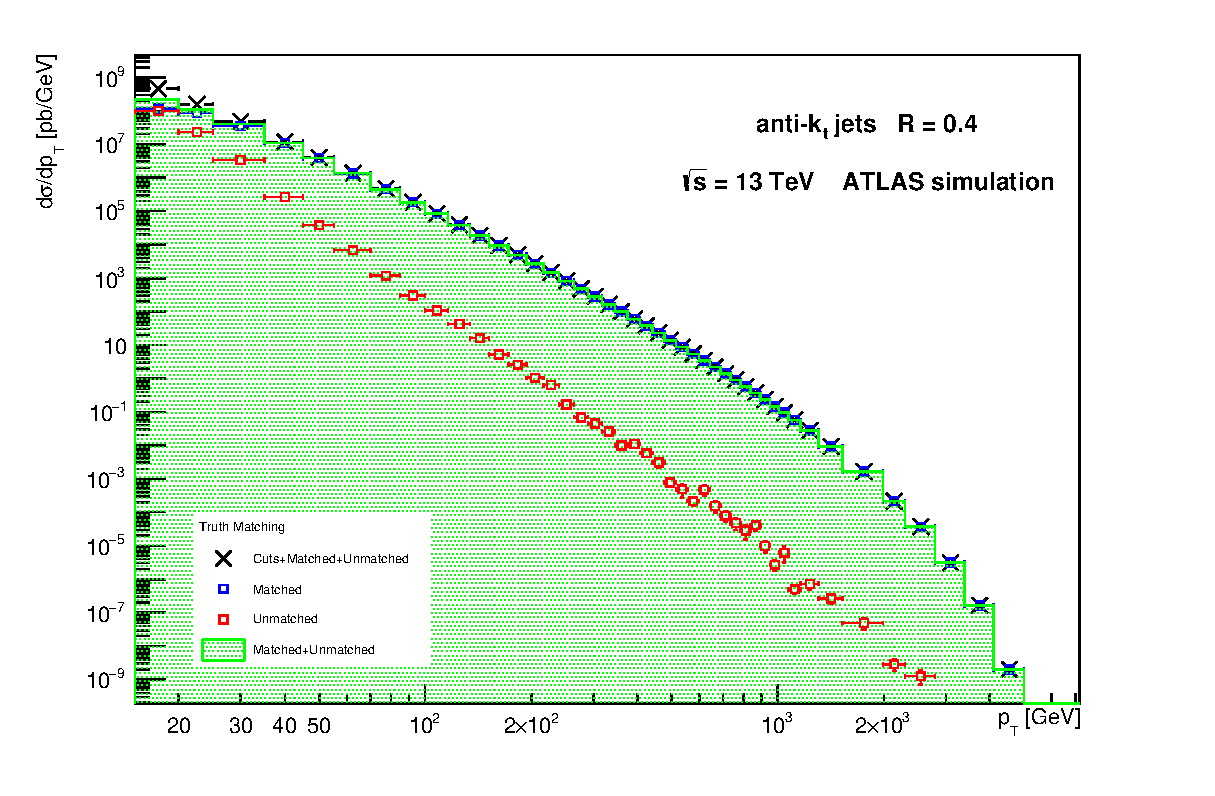
\includegraphics[width=\textwidth]{Chapter3/TruthMatching.eps}
  \caption{Results of matching procedure described in Section
  \ref{SubSec:JetMatching} demonstrated on differential cross section in $\pt$ of
  reco (top) and truth (bottom) jets. Black dots represent the original
  uncutted spectrum. The contribution of matched and unmatched jets to
  green area representing all jets which survived cutoffs is shown.}
  \label{fig:Matching}
\end{figure}

\section{Truth and Reco $\pt$ Spectra}
\label{sec:TruthAndRecoSpectra}

\begin{figure}[H]
  \centering
  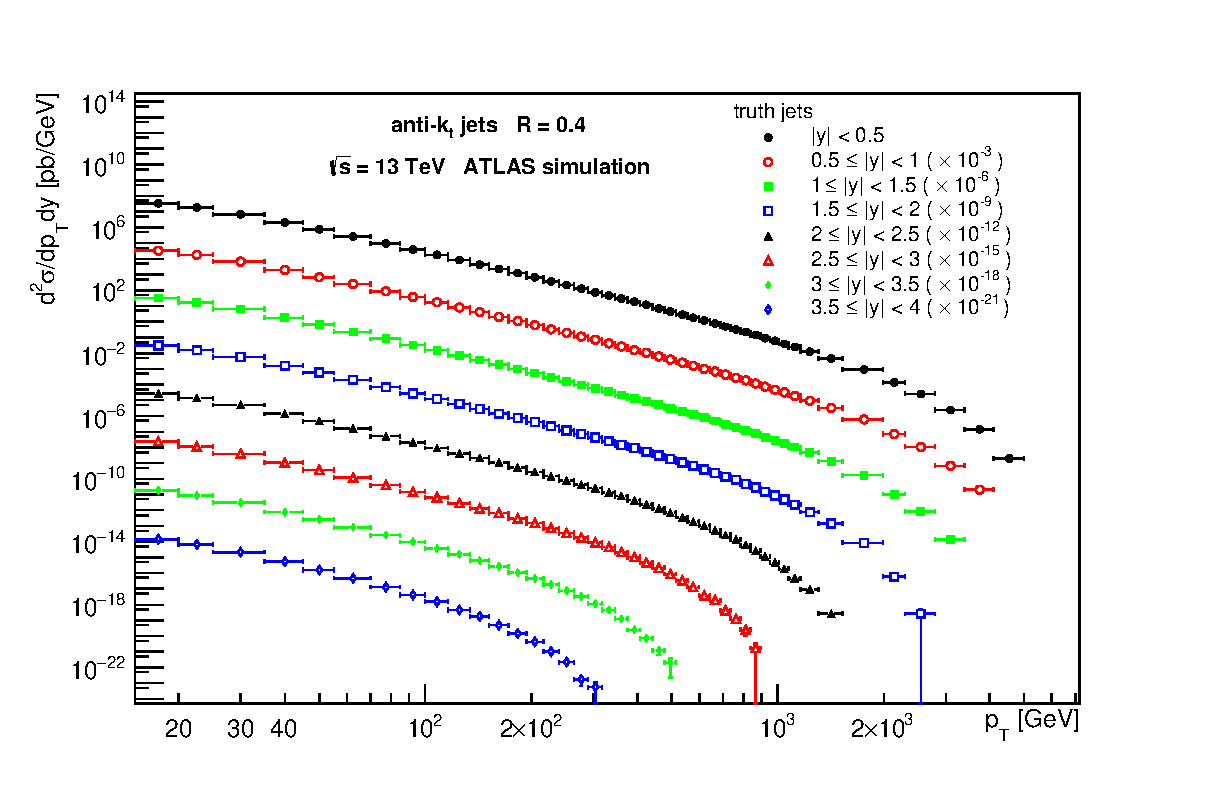
\includegraphics[width=\textwidth]{Chapter3/ptTruthAllRapidityBins.eps}
  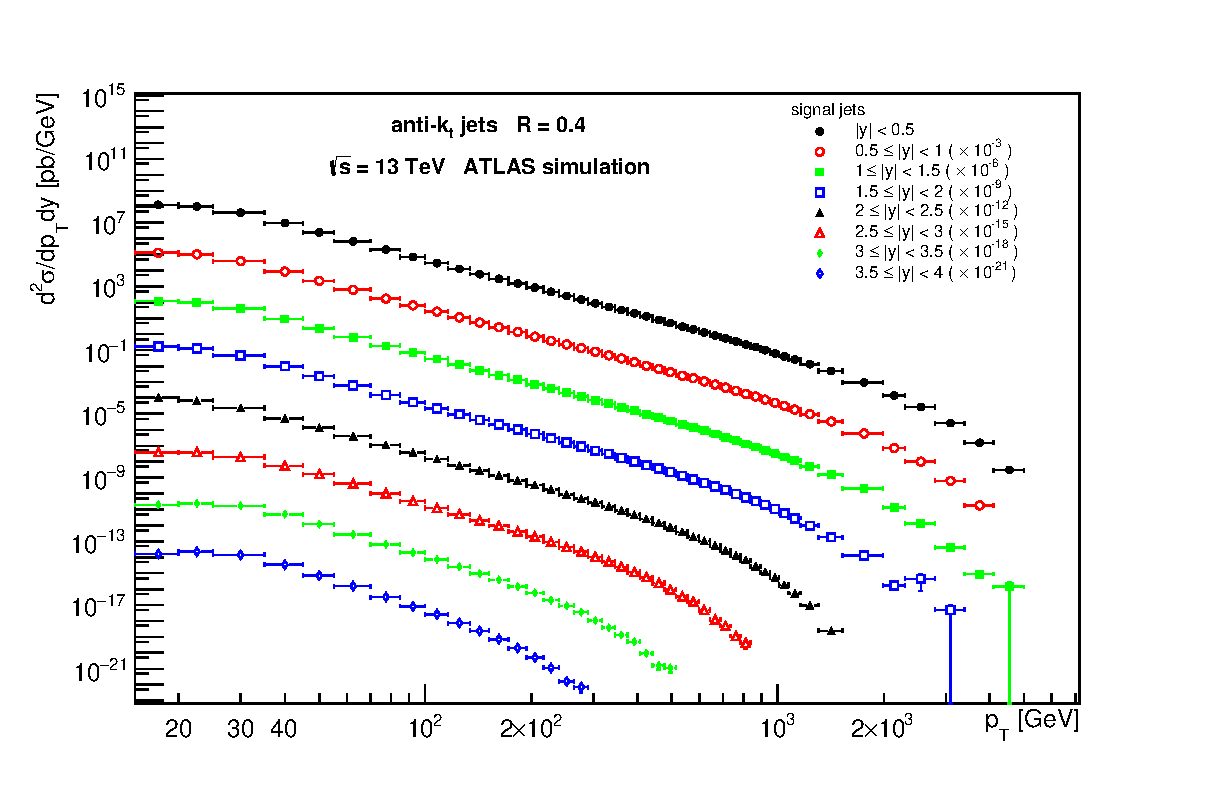
\includegraphics[width=\textwidth]{Chapter3/ptSignalAllRapidityBins.eps}
  \caption{Inclusive jet cross section of truth (top) and reco (bottom) jets as
    the function of jet $\pt$ and rapidity. For the convenience the cross
    sections for different rapidity bins are multiplied by the factor indicated
    in the legend. Jets were identified with anti-$k_t$ jet algorithm with
    $R=0.4$.}
  \label{fig:ptSpectraMasacreEverythingFuck}
\end{figure}


\begin{landscape} 
\begin{table}
  \small
  \centering
  \begin{tabular}{|c|c|>{\bfseries}c|c|c|c|c|c|c|c|c|}
    \hline
     \multicolumn{2}{|c|}{\# jets}  & ALL      & JZ0W     & JZ1W     & JZ2W     & JZ3W     & JZ4W     & JZ5W     & JZ6W     & JZ7W     \\
    \hline                                                              
    \hline                                                              
     \multicolumn{2}{|c|}{Reco}                               & 1.09e+08 & 3.11e+07 & 3.59e+07 & 6.67e+06 & 7.07e+06 & 6.28e+06 & 7.29e+06 & 7.13e+06 & 7.11e+06 \\
    \hline                                                                                          
     \multicolumn{2}{|c|}{Truth}                                & 7.28e+07 & 3.04e+06 & 3.00e+07 & 6.17e+06 & 6.91e+06 & 6.20e+06 & 6.98e+06 & 6.53e+06 & 6.25e+06 \\
    \hline                                                                                      
    \hline                                                                                      
    \multirow{4}{*}{CutPt}          & \multirow{2}{*}{Reco}   & 9.36e+06 & 3.74e+06 & 3.13e+06 & 6.50e+05 & 5.87e+05 & 4.76e+05 & 5.48e+05 & 5.52e+05 & 5.63e+05 \\
                                    &                           & 8.6 \%   & 12.0 \%  & 8.7 \%   & 9.7 \%   & 8.3 \%   & 7.6 \%   & 7.5 \%   & 7.7 \%   & 7.9 \%   \\
    \cline{2-11}                                                                                
                                    & \multirow{2}{*}{Truth}    & 4.70e+07 & 3.00e+06 & 2.20e+07 & 3.86e+06 & 4.00e+06 & 3.42e+06 & 3.74e+06 & 3.43e+06 & 3.23e+06 \\
                                    &                           & 64.6 \%  & 98.7 \%  & 73.1 \%  & 62.6 \%  & 57.8 \%  & 55.1 \%  & 53.6 \%  & 52.5 \%  & 51.6 \%  \\
    \hline                                                                                      
    \hline                                                                                      
    \multirow{4}{*}{Cuty}           & \multirow{2}{*}{Reco}   & 3.43e+06 & 1.19e+06 & 1.29e+06 & 1.42e+05 & 1.28e+05 & 1.03e+05 & 1.16e+05 & 1.10e+05 & 1.08e+05 \\
                                    &                           & 3.1 \%   & 3.8 \%   & 3.6 \%   & 2.1 \%   & 1.8 \%   & 1.6 \%   & 1.6 \%   & 1.5 \%   & 1.5 \%   \\
    \cline{2-11}                                                                                    
                                    & \multirow{2}{*}{Truth}    & 5.06e+05 & 3.04e+03 & 3.19e+05 & 4.54e+04 & 3.79e+04 & 2.88e+04 & 2.78e+04 & 2.22e+04 & 1.83e+04 \\
                                    &                           & 0.7 \%   & 0.1 \%   & 1.1 \%   & 0.7 \%   & 0.5 \%   & 0.5 \%   & 0.4 \%   & 0.3 \%   & 0.3 \%   \\
    \hline                                                                                      
    \hline                                                                                      
    \multirow{4}{*}{Cut0jet}        & \multirow{2}{*}{Reco}   & 2.64e+07 & 2.59e+07 & 5.70e+05 & 0.00e+00 & 0.00e+00 & 0.00e+00 & 0.00e+00 & 0.00e+00 & 0.00e+00 \\
                                    &                           & 24.2 \%  & 83.2 \%  & 1.6 \%   & 0.0 \%   & 0.0 \%   & 0.0 \%   & 0.0 \%   & 0.0 \%   & 0.0 \%   \\
    \cline{2-11}                                                                                    
                                    & \multirow{2}{*}{Truth}    & 0.00e+00 & 0.00e+00 & 0.00e+00 & 0.00e+00 & 0.00e+00 & 0.00e+00 & 0.00e+00 & 0.00e+00 & 0.00e+00 \\
                                    &                           & 0.0 \%   & 0.0 \%   & 0.0 \%   & 0.0 \%   & 0.0 \%   & 0.0 \%   & 0.0 \%   & 0.0 \%   & 0.0 \%   \\
    \hline                                                                                      
    \hline                                                                                      
    \multirow{4}{*}{CutLR}          & \multirow{2}{*}{Reco}   & 4.09e+06 & 2.38e+05 & 3.82e+06 & 2.99e+04 & 7.07e+03 & 2.33e+03 & 1.63e+03 & 7.14e+02 & 6.31e+02 \\
                                    &                           & 3.7 \%   & 0.8 \%   & 10.6 \%  & 0.4 \%   & 0.1 \%   & 0.0 \%   & 0.0 \%   & 0.0 \%   & 0.0 \%   \\
    \cline{2-11}                                                                                    
                                    & \multirow{2}{*}{Truth}    & 5.40e+05 & 2.19e+04 & 4.96e+05 & 1.82e+04 & 4.45e+03 & 1.33e+03 & 9.03e+02 & 4.37e+02 & 2.78e+02 \\
                                    &                           & 0.7 \%   & 0.7 \%   & 1.7 \%   & 0.3 \%   & 0.1 \%   & 0.0 \%   & 0.0 \%   & 0.0 \%   & 0.0 \%   \\
    \hline                                                                                      
    \hline                                                                                      
    \multirow{4}{*}{Matched}        & \multirow{2}{*}{Reco}   & 2.17e+07 & 7.62e+03 & 6.03e+06 & 1.95e+06 & 2.54e+06 & 2.46e+06 & 2.88e+06 & 2.78e+06 & 2.72e+06 \\
                                    &                           & 19.8 \%  & 0.0 \%   & 16.8 \%  & 29.3 \%  & 36.0 \%  & 39.1 \%  & 39.5 \%  & 38.9 \%  & 38.2 \%  \\
    \cline{2-11}                                                                                    
                                    & \multirow{2}{*}{Truth}    & 2.17e+07 & 7.62e+03 & 6.03e+06 & 1.95e+06 & 2.54e+06 & 2.46e+06 & 2.88e+06 & 2.78e+06 & 2.72e+06 \\
                                    &                           & 29.8 \%  & 0.3 \%   & 20.1 \%  & 31.7 \%  & 36.8 \%  & 39.6 \%  & 41.3 \%  & 42.5 \%  & 43.5 \%  \\
    \hline                                                                                      
    \hline                                                                                      
    \multirow{4}{*}{Unmatched}      & \multirow{2}{*}{Reco}   & 4.42e+07 & 5.36e+04 & 2.10e+07 & 3.89e+06 & 3.81e+06 & 3.24e+06 & 3.75e+06 & 3.69e+06 & 3.72e+06 \\
                                    &                           & 40.5 \%  & 0.2 \%   & 58.6 \%  & 58.4 \%  & 53.8 \%  & 51.6 \%  & 51.4 \%  & 51.8 \%  & 52.3 \%  \\
    \cline{2-11}                                                                                    
                                    & \multirow{2}{*}{Truth}    & 3.07e+06 & 6.18e+03 & 1.25e+06 & 2.89e+05 & 3.29e+05 & 2.95e+05 & 3.29e+05 & 3.03e+05 & 2.88e+05 \\
                                    &                           & 4.2 \%   & 0.2 \%   & 4.2 \%   & 4.7 \%   & 4.8 \%   & 4.8 \%   & 4.7 \%   & 4.6 \%   & 4.6 \%   \\
    \hline
  \end{tabular}
  \caption{Statistics for matching and cutting procedures described in Sections
    \ref{SubSec:JetCuts} and \ref{SubSec:JetMatching} displayed for all jets and for
    individual JZXW samples defined in Table \ref{tab:JZXW}. At the top, there is
    number of initial reco and truth jets respectively. For each cut, there is
    shown the number of jets, which were killed by it, and their relative number
    according to the original number of reco or truth jets respectively.
    Last two lines show the statistics of matching procedure including number of
    jets which were (un)matched.}
  \label{tab:CutAndMatchingEfficiency}
\end{table} 
\end{landscape}

\chapter{Unfolding}
\label{App:UnfoldingResults}

\section{Matching Efficiency}
\label{sec:MatchingEfficiency}

\begin{figure}[H]
  \centering
  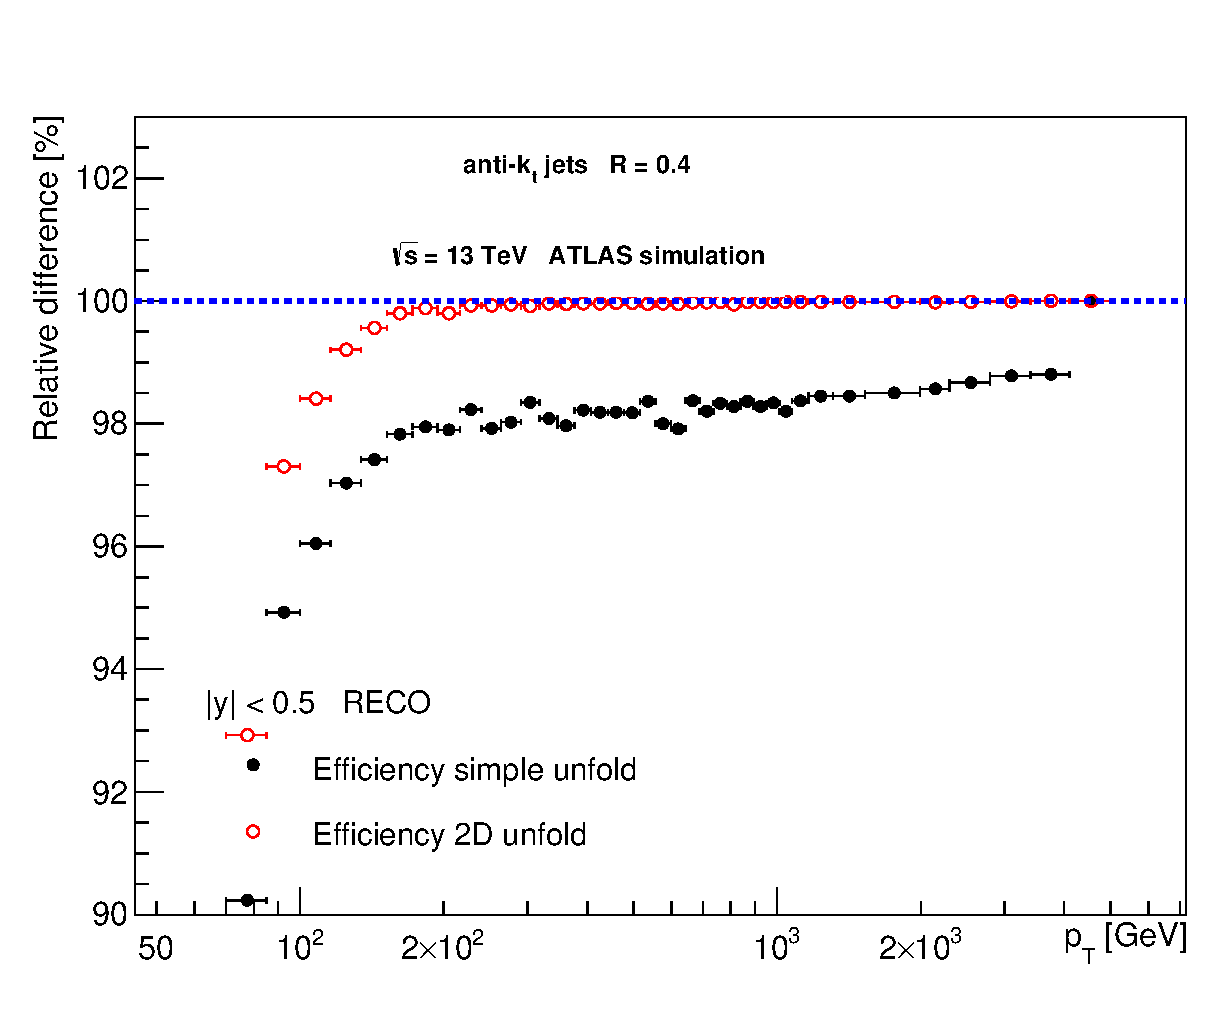
\includegraphics[width=0.49\textwidth]{{Chapter3/MatchEffSimpe2DSignal0Compare}.eps}
  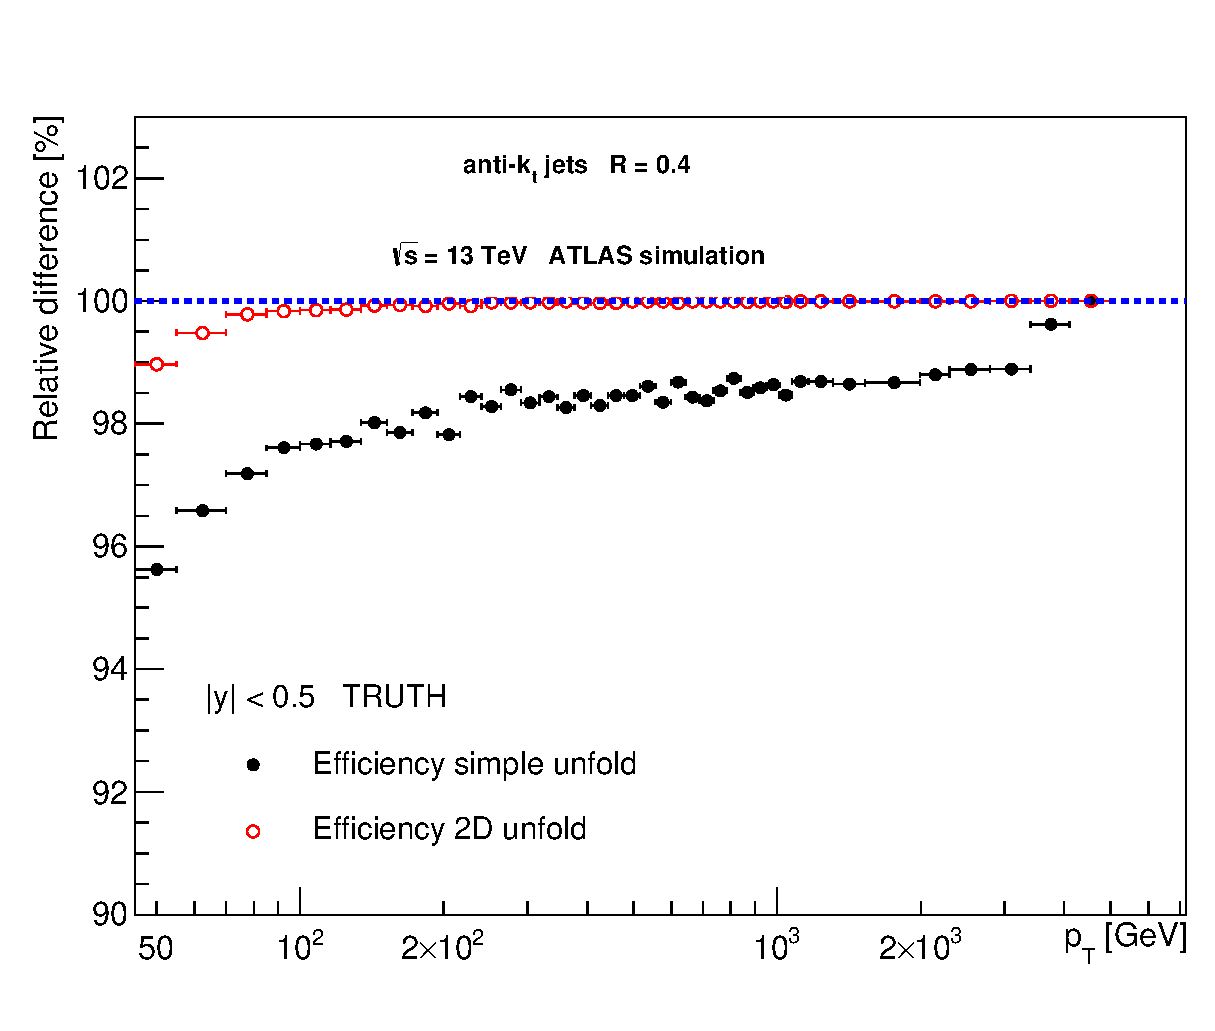
\includegraphics[width=0.49\textwidth]{{Chapter3/MatchEffSimpe2DTruth0Compare}.eps}
  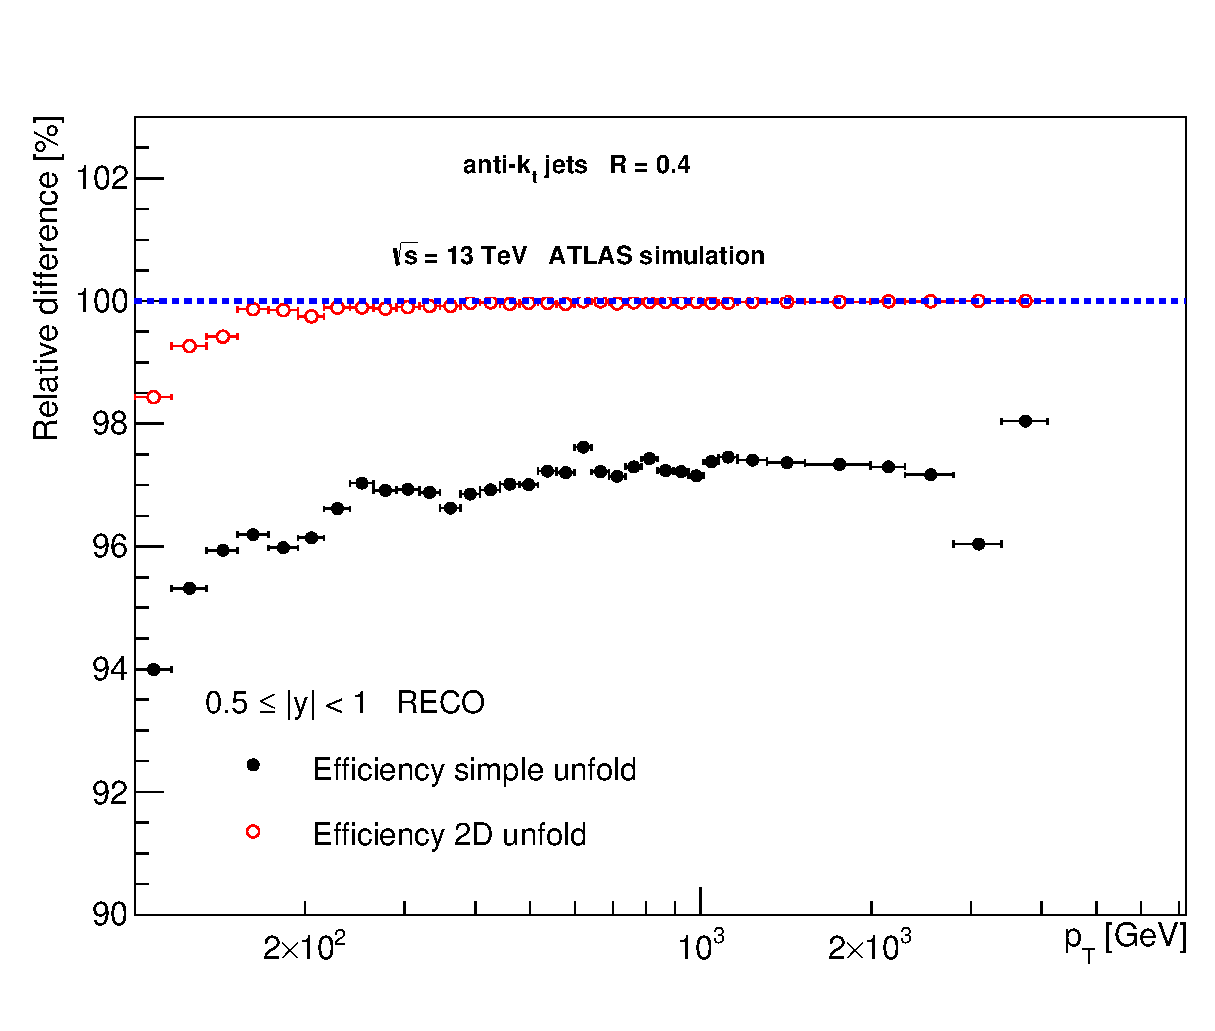
\includegraphics[width=0.49\textwidth]{{Chapter3/MatchEffSimpe2DSignal1Compare}.eps}
  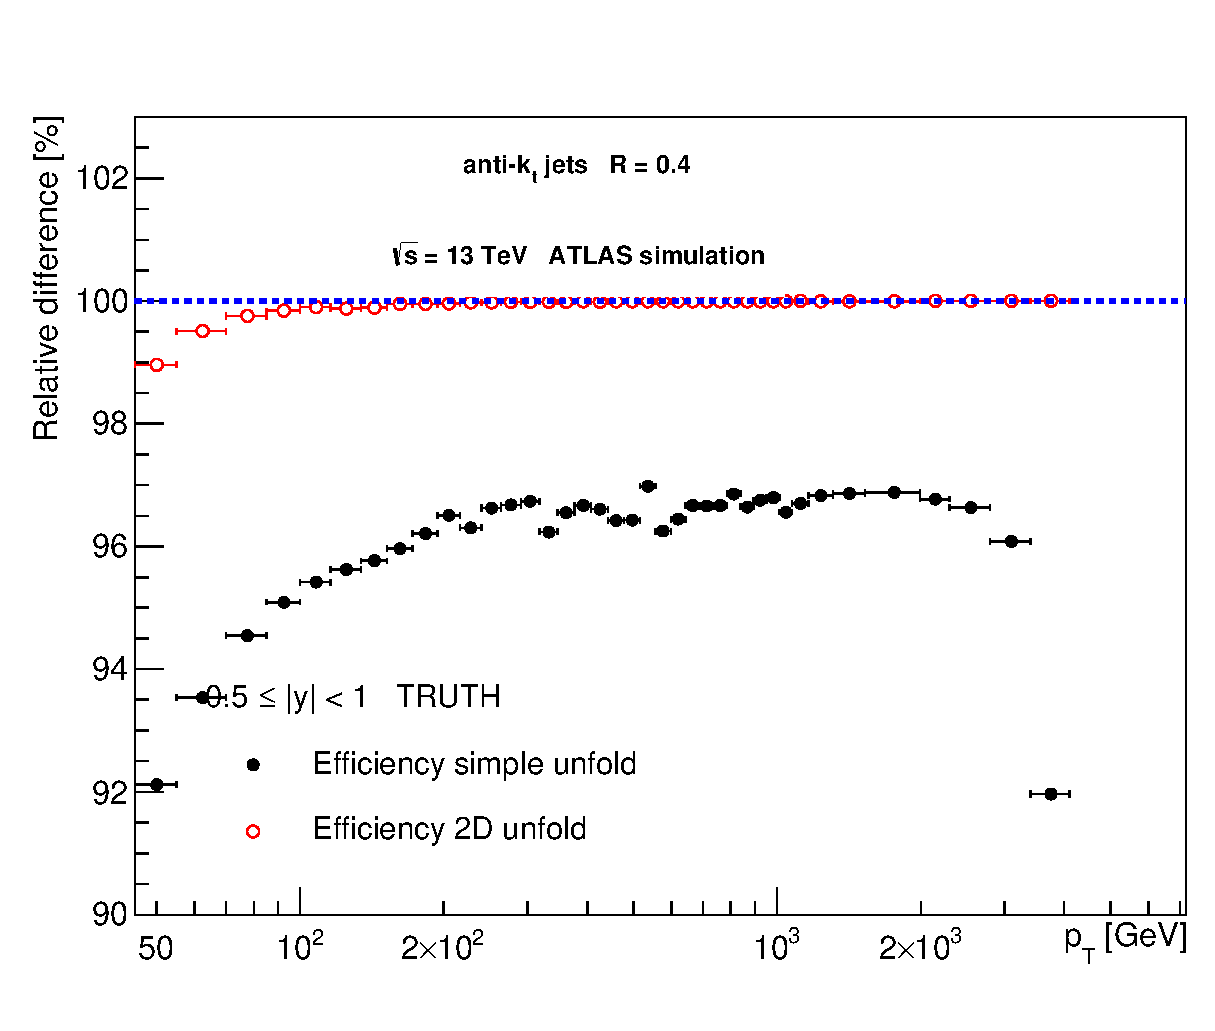
\includegraphics[width=0.49\textwidth]{{Chapter3/MatchEffSimpe2DTruth1Compare}.eps}
  \caption{Comparison of matching efficiencies of simple and 2D unfolding for
  $|y| < 0.5$ (top) and $0.5 \leq |y| < 1$ (bottom) rapidity bins. Matching
  efficiencies are shown for both reco jets (left) and truth jets (right). }
\end{figure}

\begin{figure}[p]
  \centering
  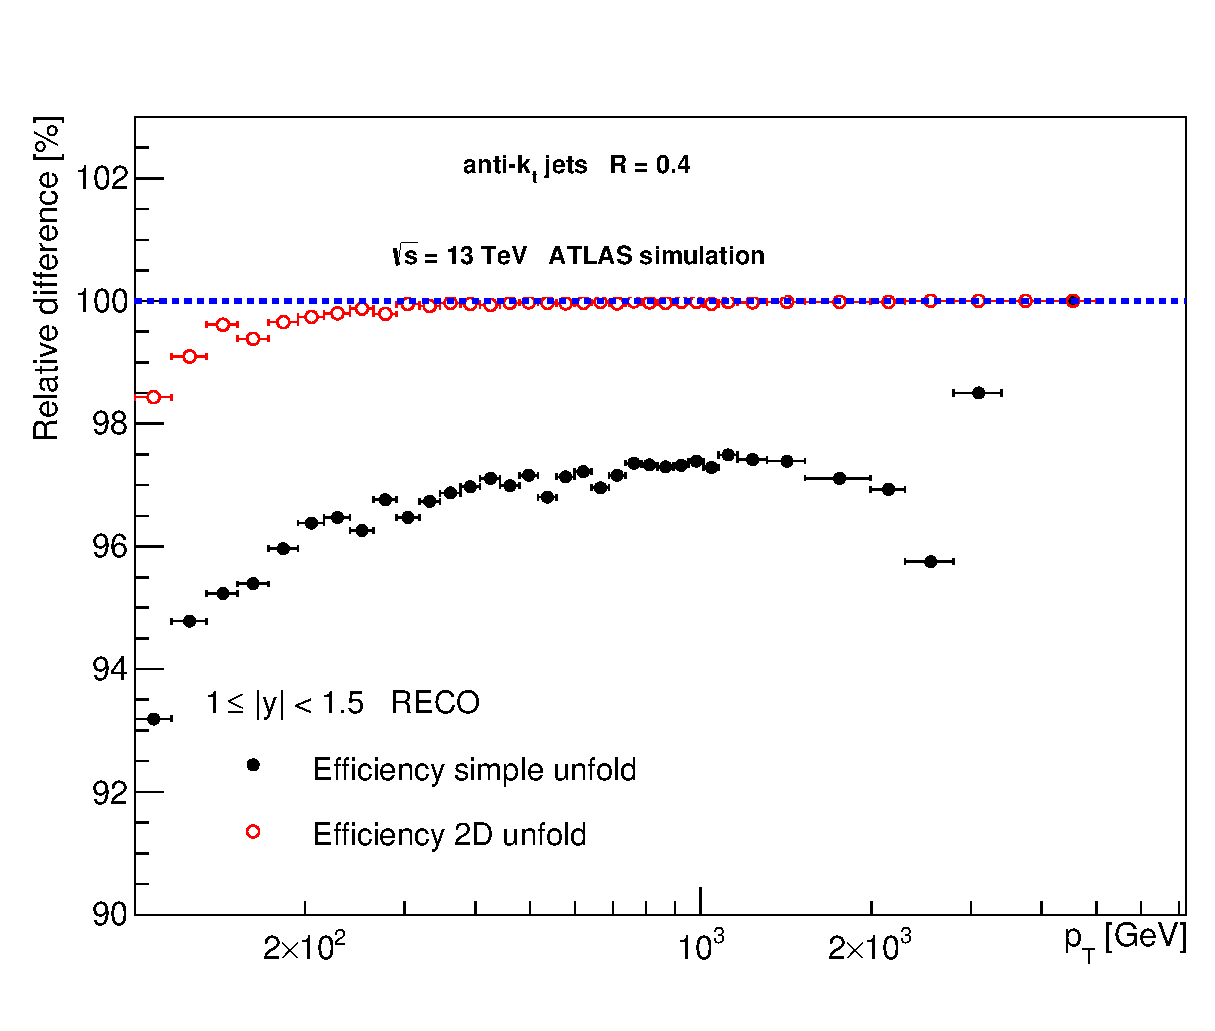
\includegraphics[width=0.49\textwidth]{{Chapter3/MatchEffSimpe2DSignal2Compare}.eps}
   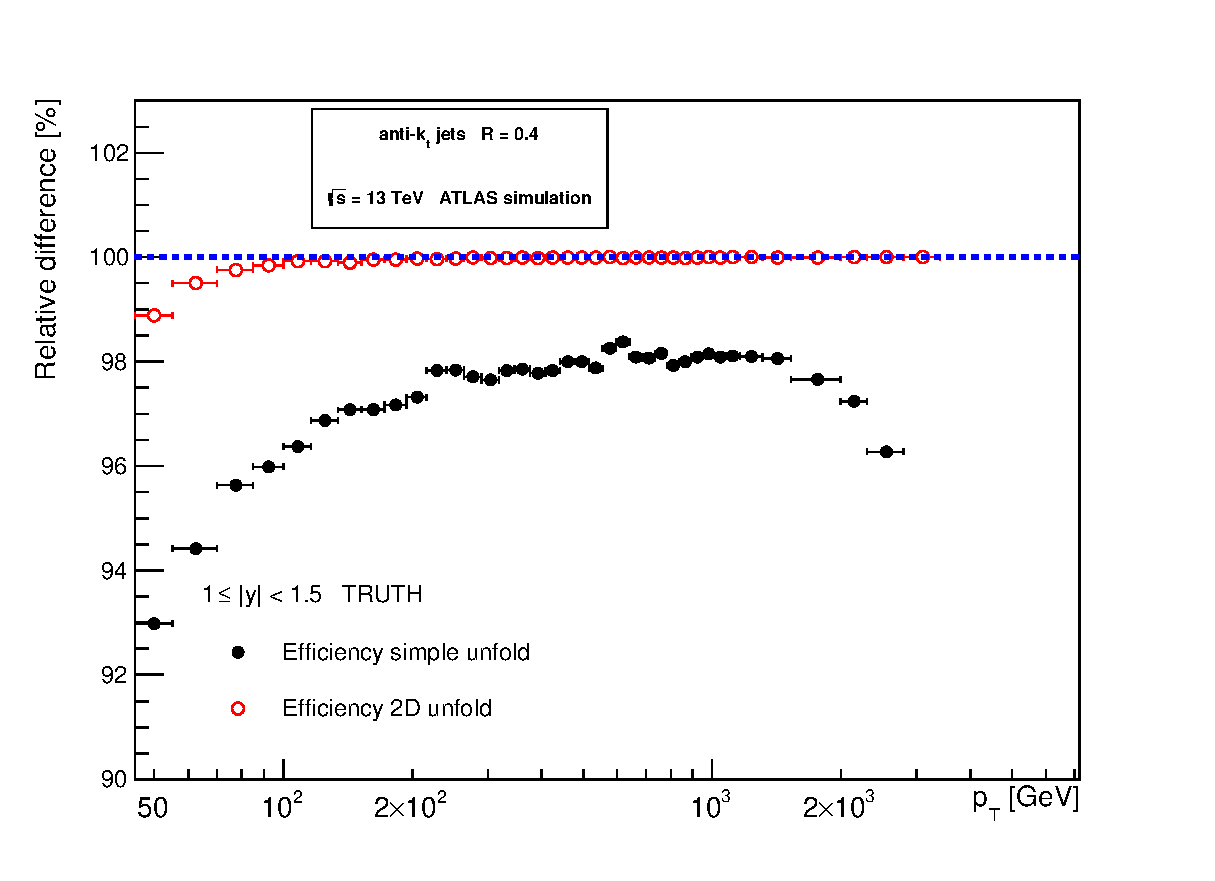
\includegraphics[width=0.49\textwidth]{{Chapter3/MatchEffSimpe2DTruth2Compare}.eps}
  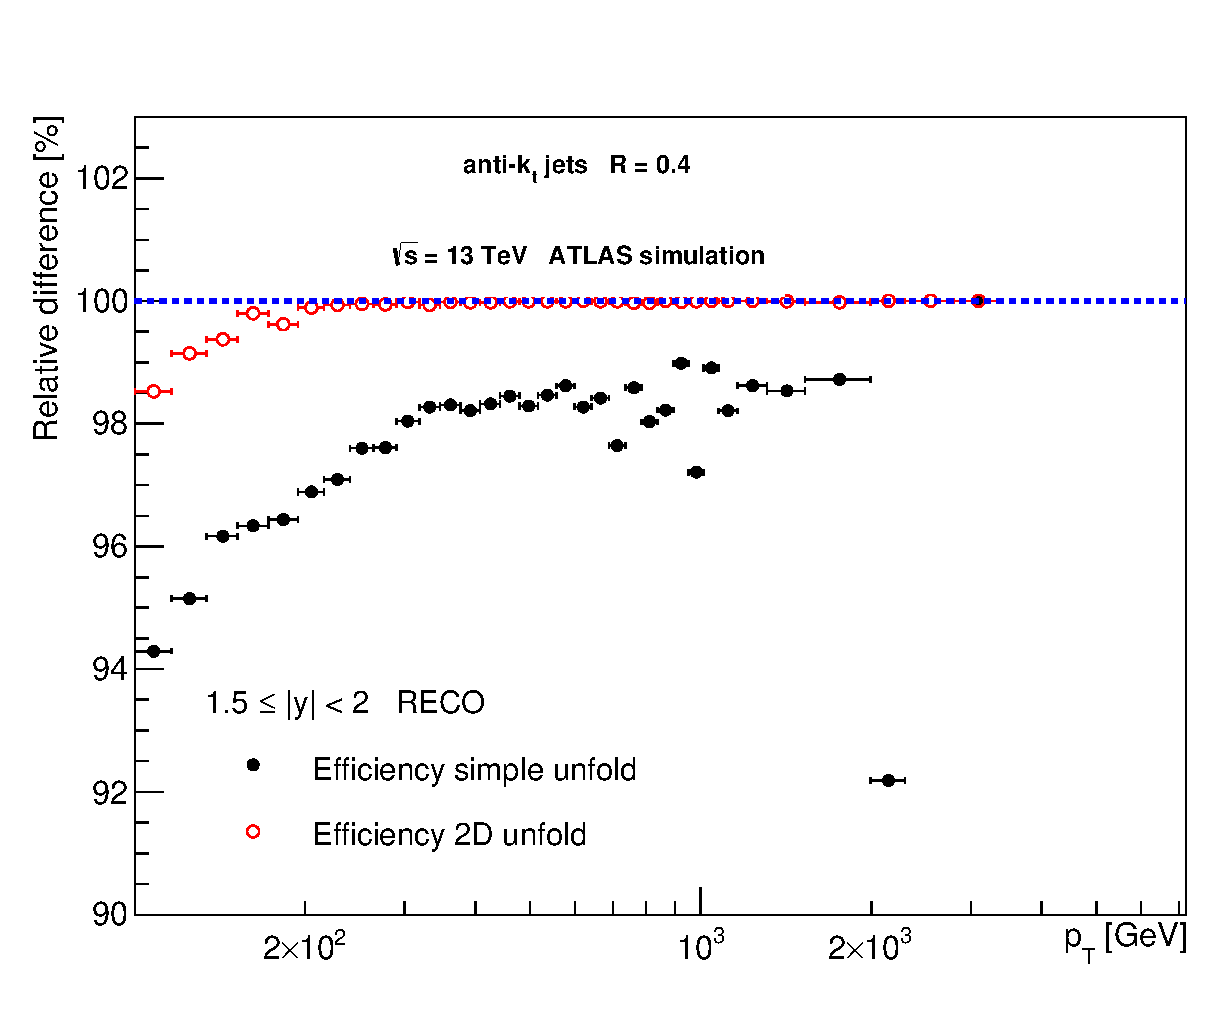
\includegraphics[width=0.49\textwidth]{{Chapter3/MatchEffSimpe2DSignal3Compare}.eps}
   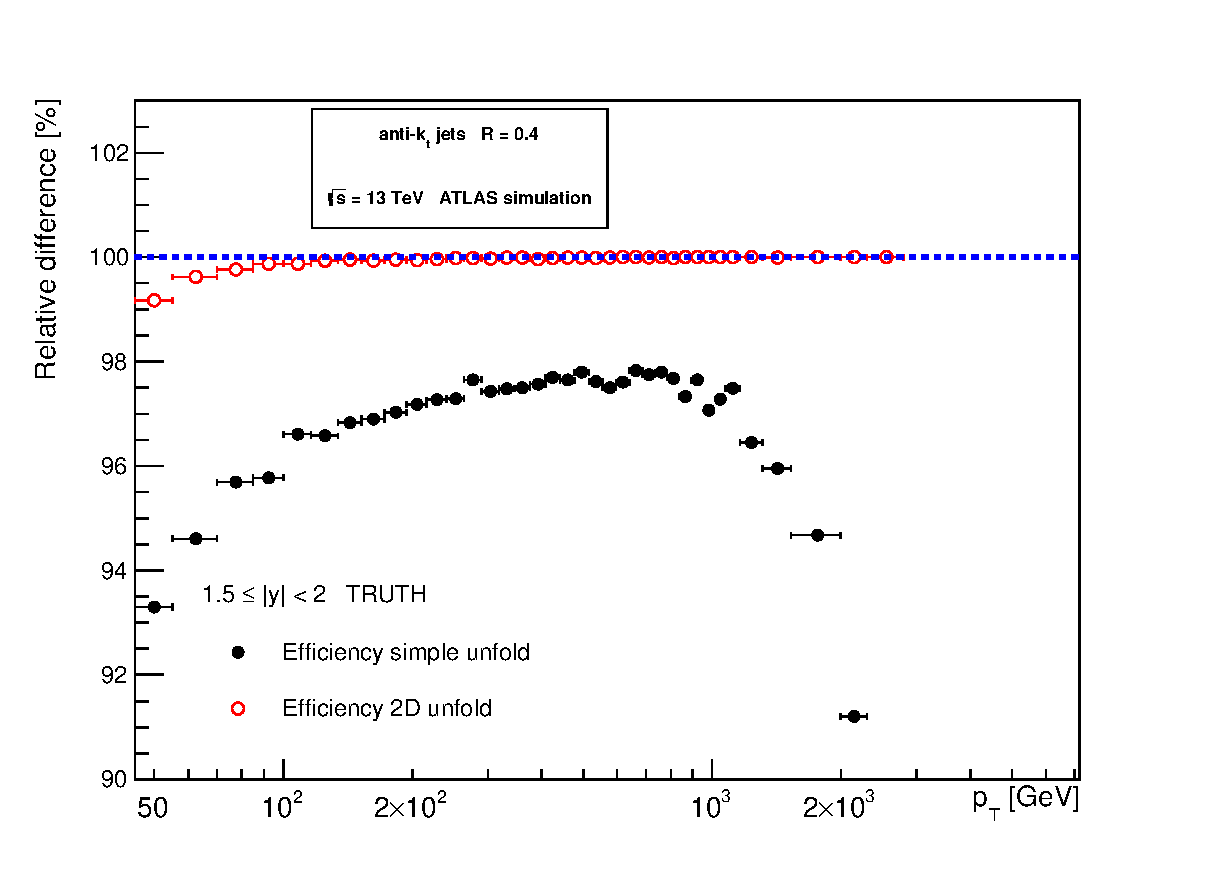
\includegraphics[width=0.49\textwidth]{{Chapter3/MatchEffSimpe2DTruth3Compare}.eps}
  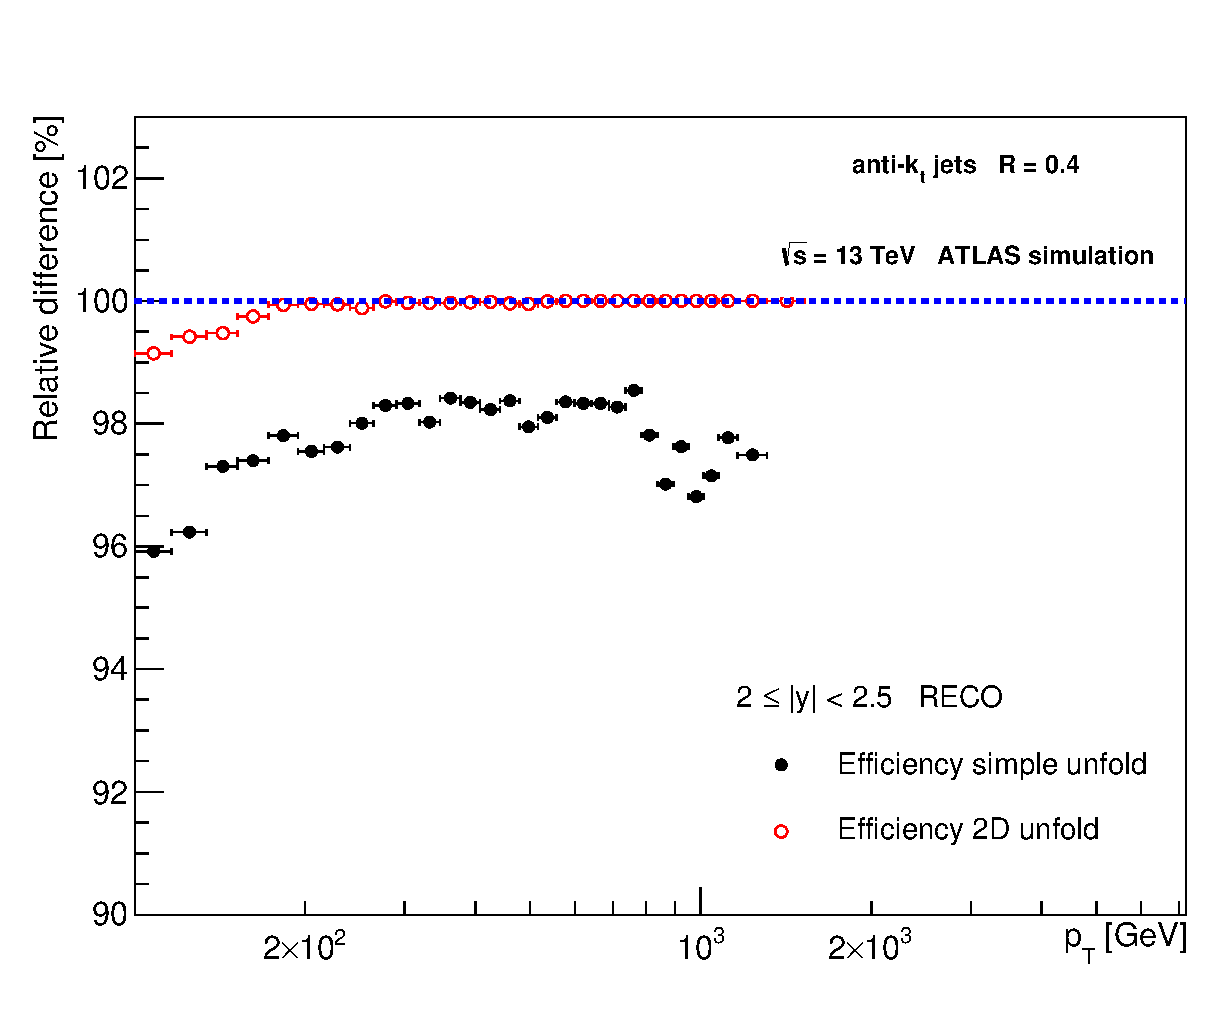
\includegraphics[width=0.49\textwidth]{{Chapter3/MatchEffSimpe2DSignal4Compare}.eps}
   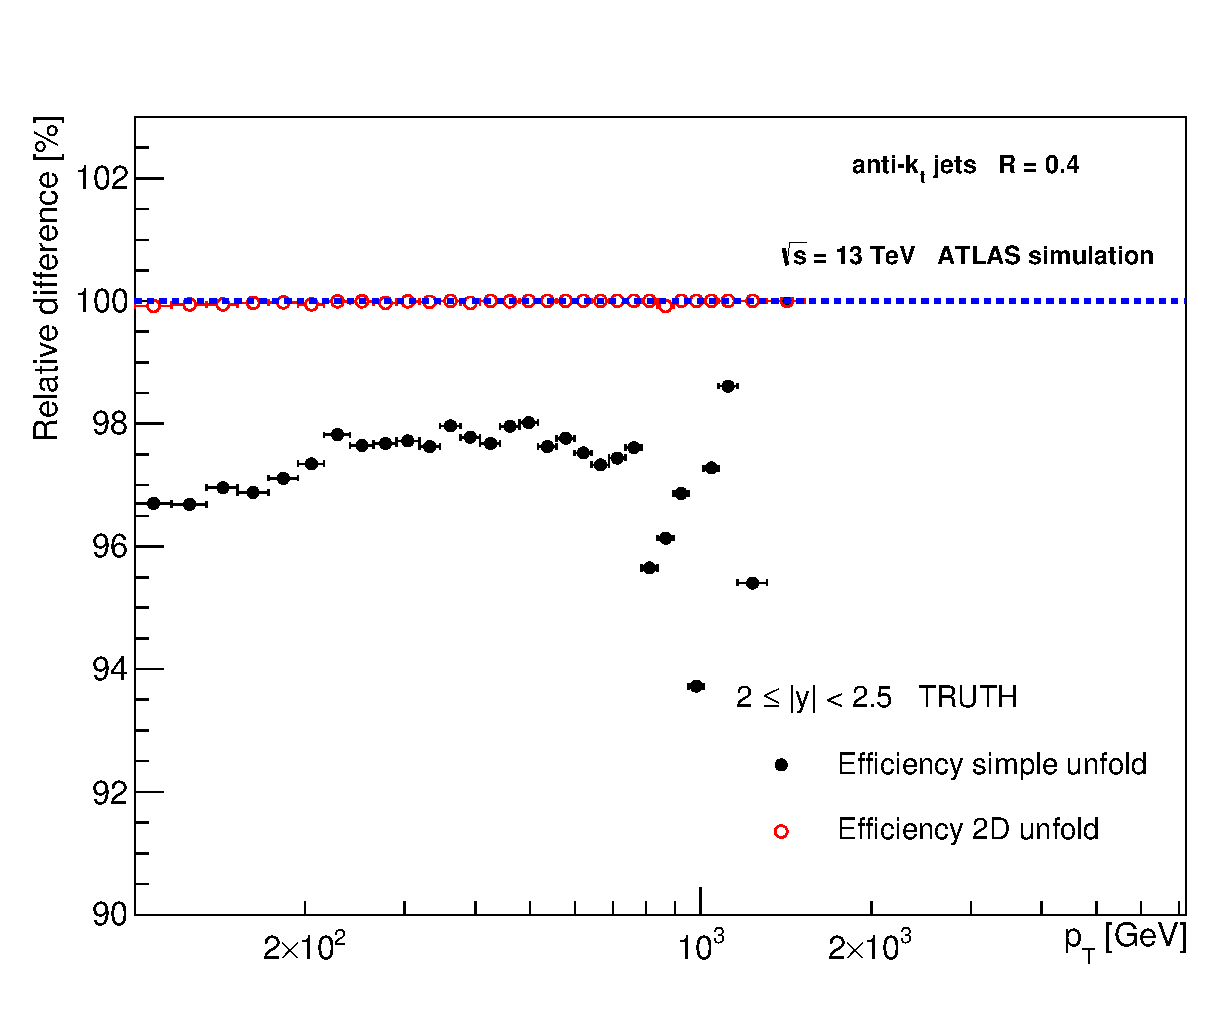
\includegraphics[width=0.49\textwidth]{{Chapter3/MatchEffSimpe2DTruth4Compare}.eps}
  \caption{Comparison of matching efficiencies of simple and 2D unfolding for
  $1 \leq |y| < 1.5$ (top), $1.5 \leq |y| < 2$ and $2 \leq |y| < 2.5$ (bottom)
  rapidity bins. Matching efficiencies are shown for both reco jets (left) and truth
  jets (right). }
\end{figure}

\begin{figure}[p]
  \centering
  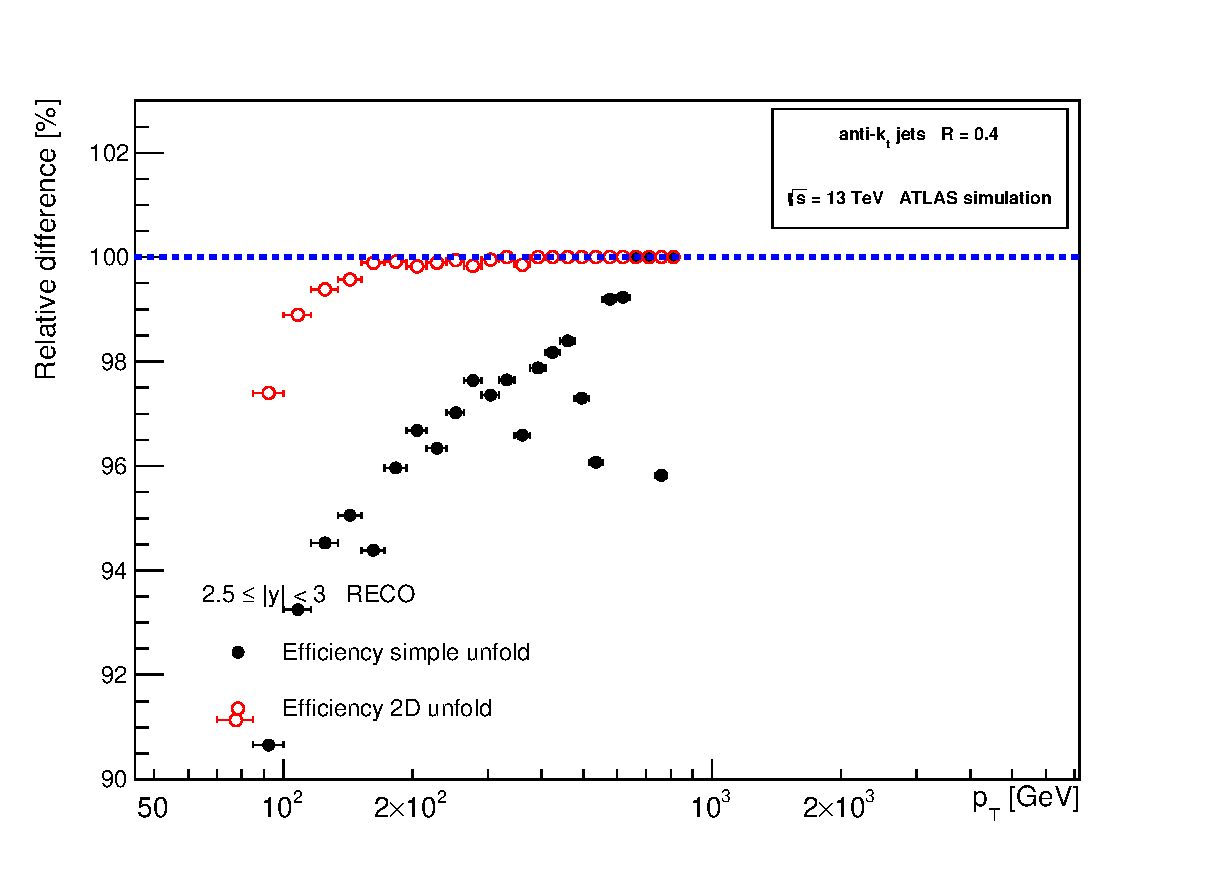
\includegraphics[width=0.49\textwidth]{{Chapter3/MatchEffSimpe2DSignal5Compare}.eps}
   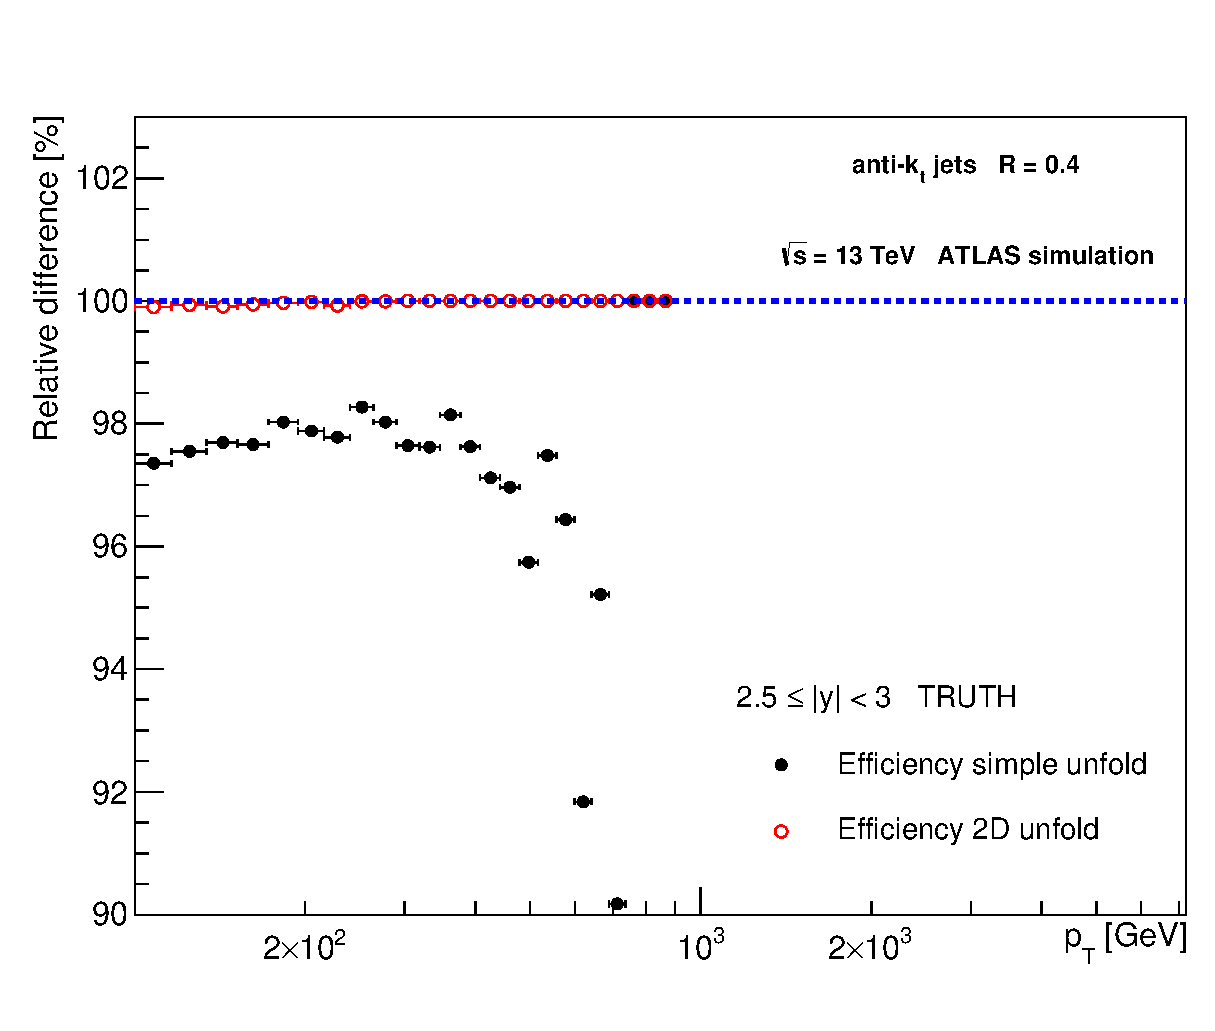
\includegraphics[width=0.49\textwidth]{{Chapter3/MatchEffSimpe2DTruth5Compare}.eps}
  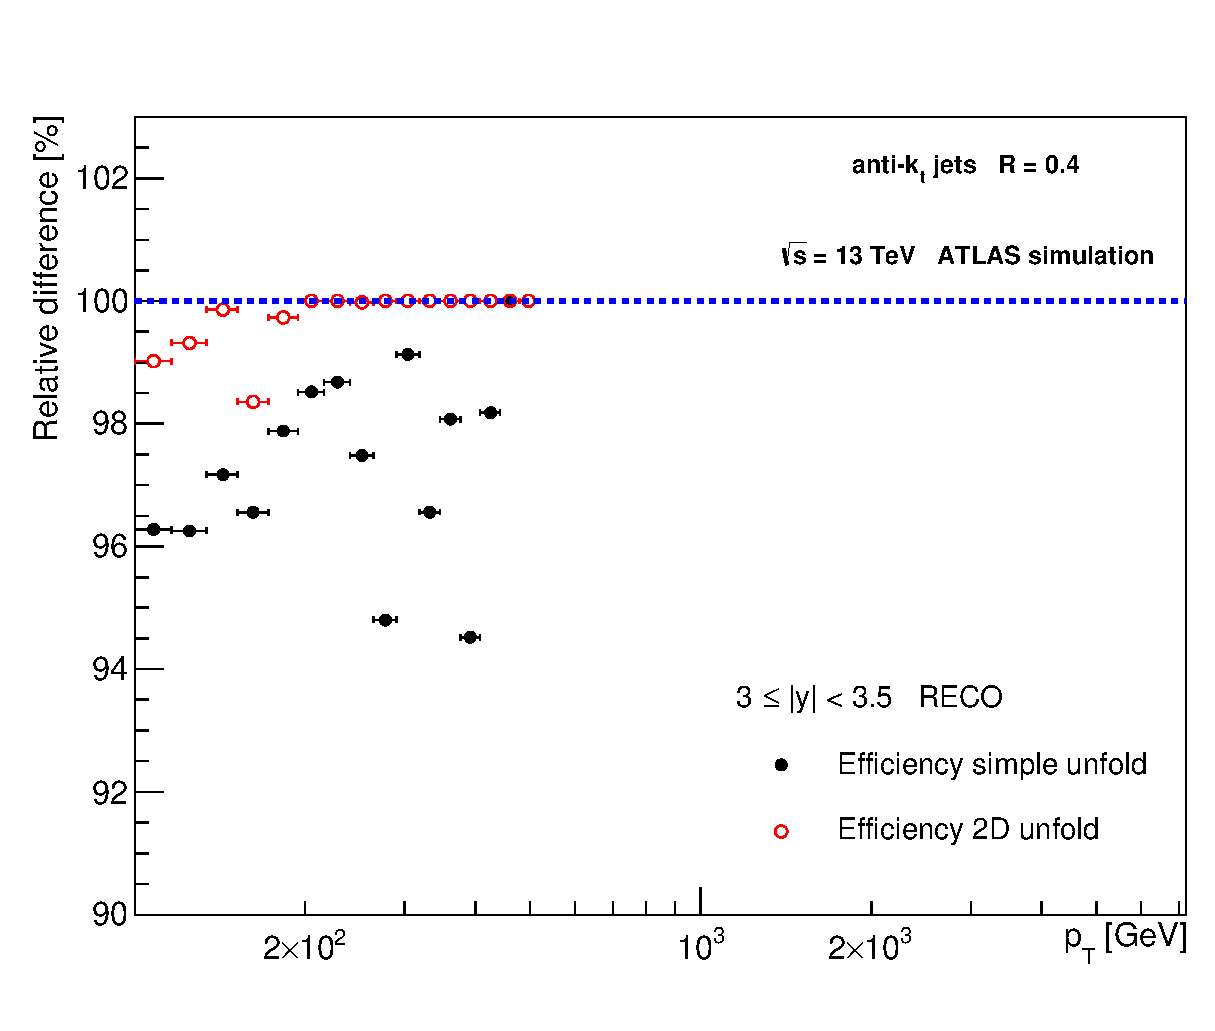
\includegraphics[width=0.49\textwidth]{{Chapter3/MatchEffSimpe2DSignal6Compare}.eps}
   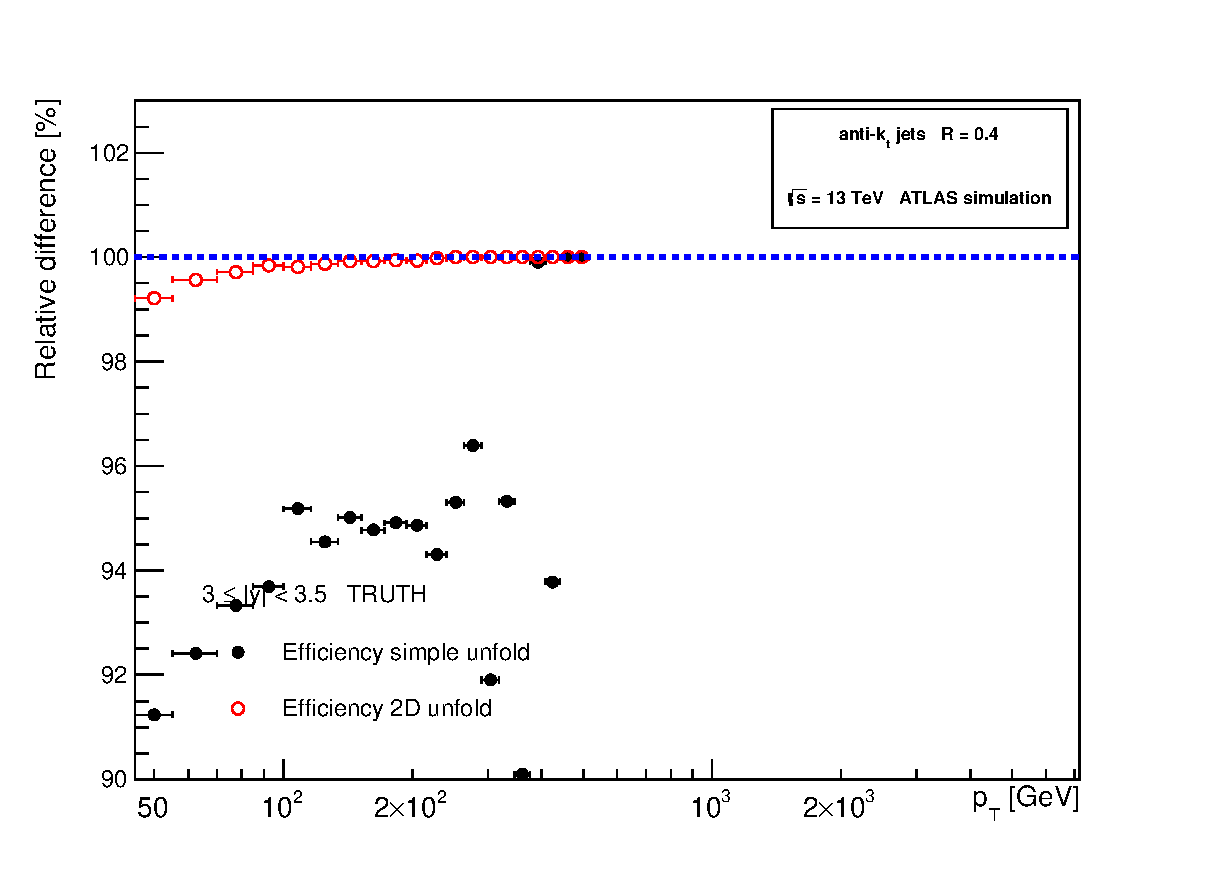
\includegraphics[width=0.49\textwidth]{{Chapter3/MatchEffSimpe2DTruth6Compare}.eps}
  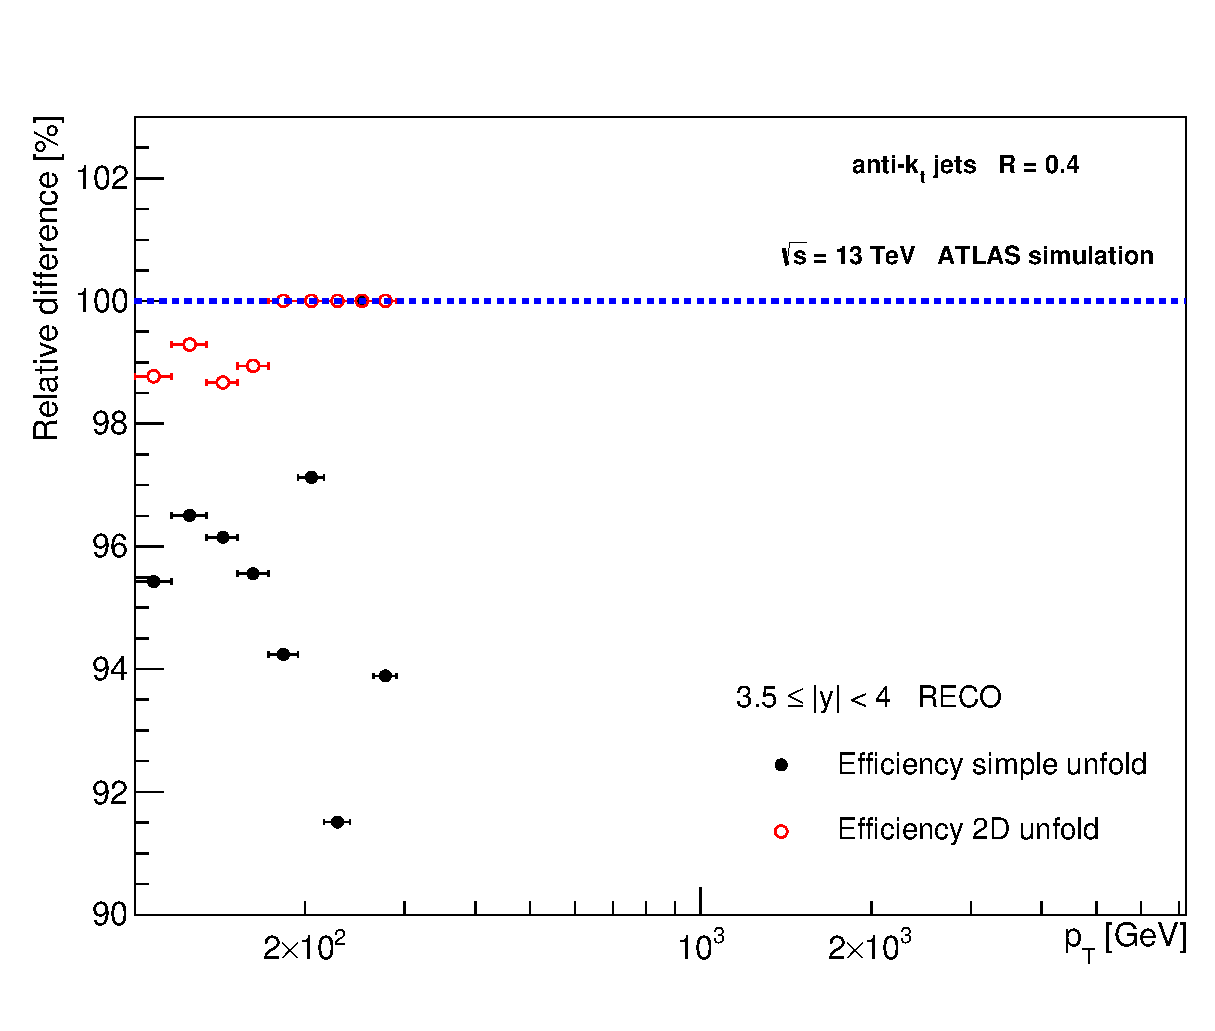
\includegraphics[width=0.49\textwidth]{{Chapter3/MatchEffSimpe2DSignal7Compare}.eps}
   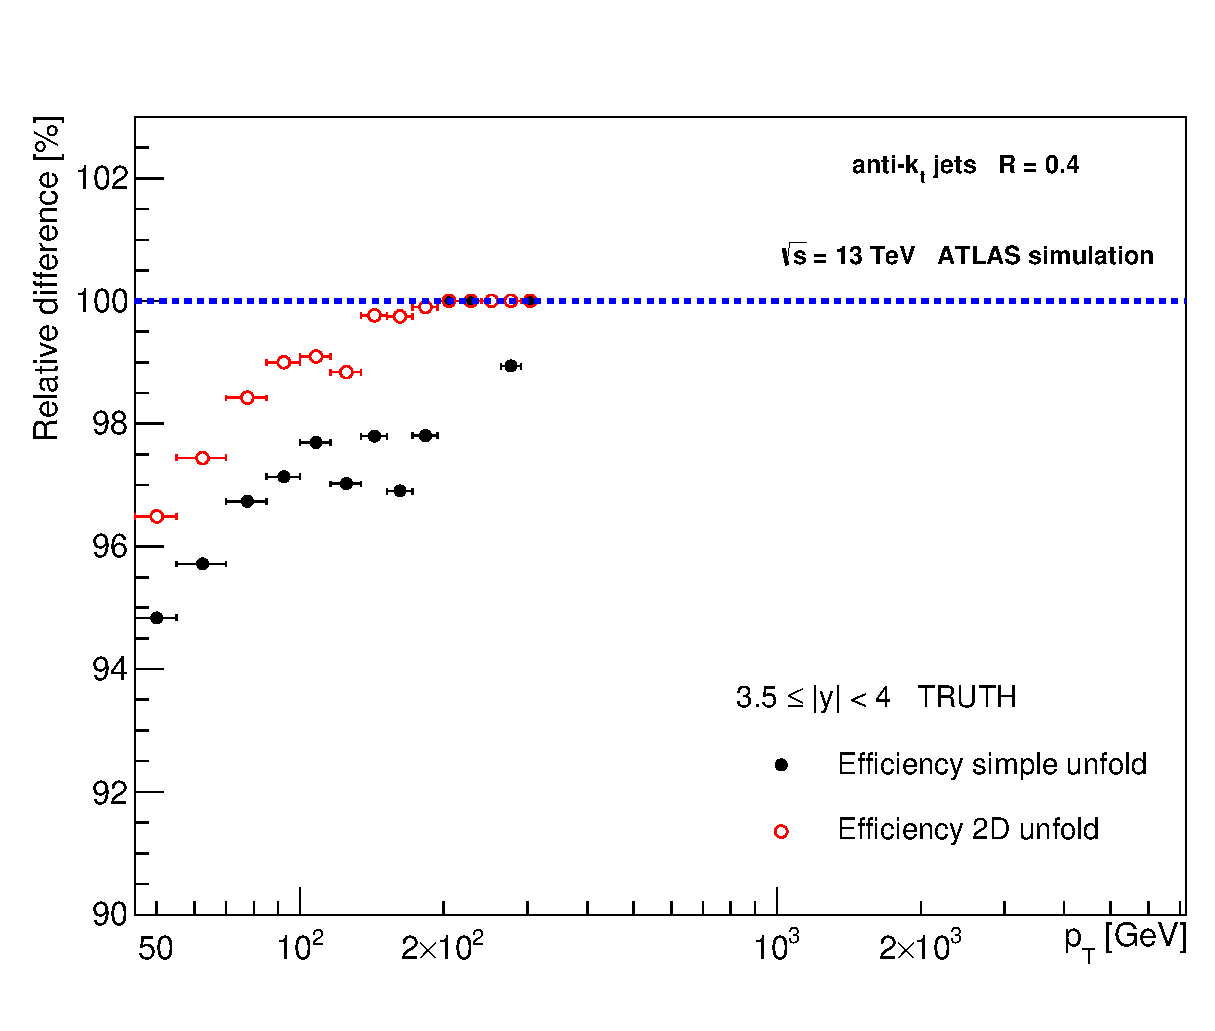
\includegraphics[width=0.49\textwidth]{{Chapter3/MatchEffSimpe2DTruth7Compare}.eps}
  \caption{Comparison of matching efficiencies of simple and 2D unfolding for
  $2.5 \leq |y| < 3$ (top), $3 \leq |y| < 3.5$ and $3.5 \leq |y| < 4$ (bottom)
  rapidity bins. Matching efficiencies are shown for both reco jets (left) and truth
  jets (right). }
\end{figure}

\section{Slices in Unfolding Matrix}
\label{sec:UnfoldingMatrixSlices}

\begin{figure}[H]
  \centering
  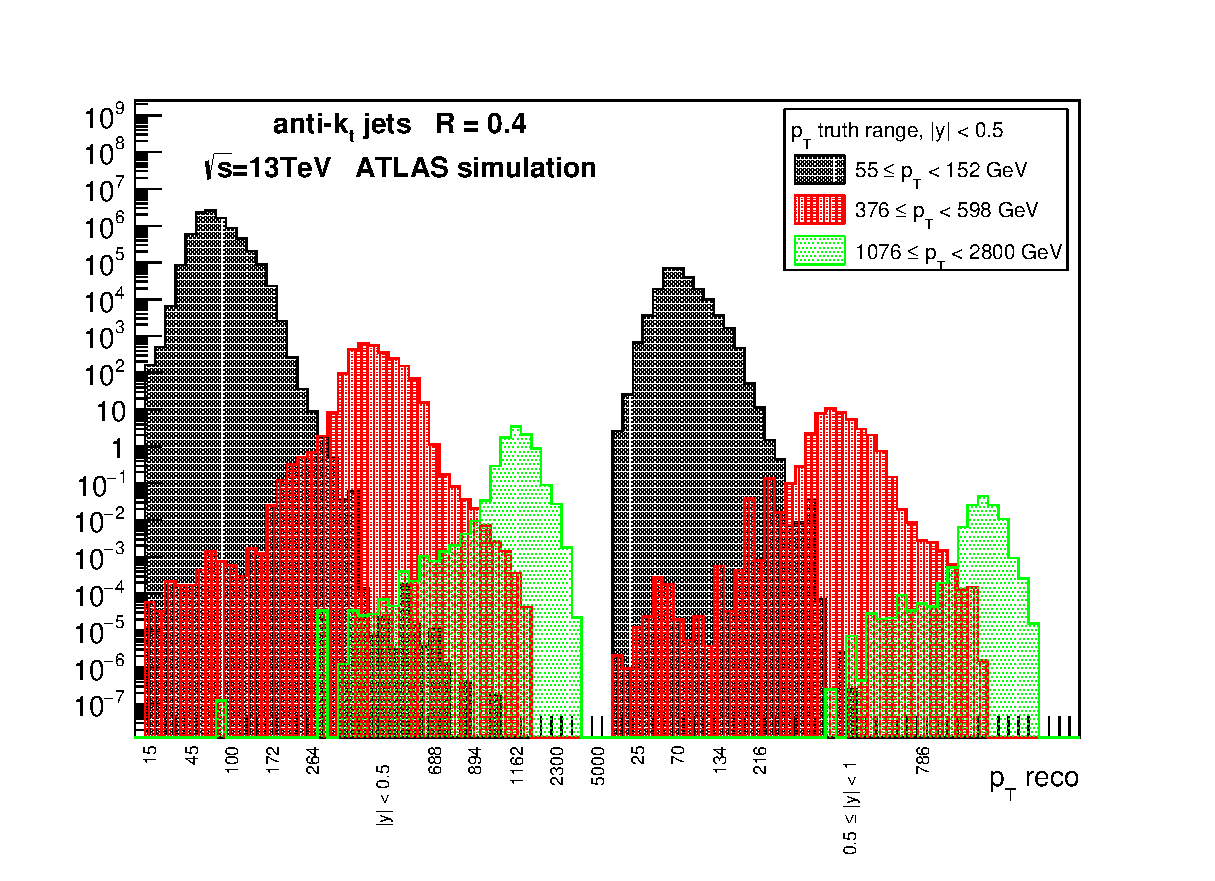
\includegraphics[width=0.49\textwidth]{{Chapter3/UnfoldMatrixSlices00}.eps}
  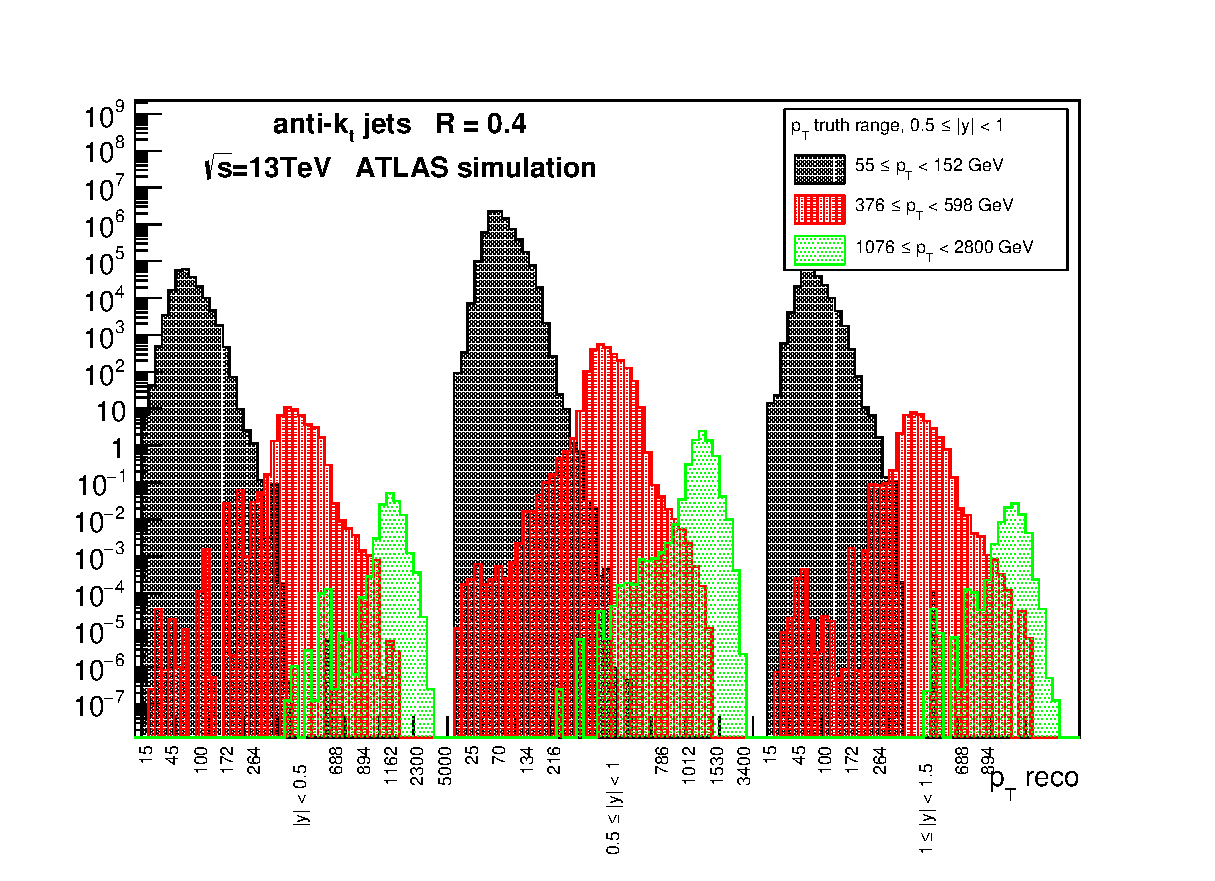
\includegraphics[width=0.49\textwidth]{{Chapter3/UnfoldMatrixSlices11}.eps}
  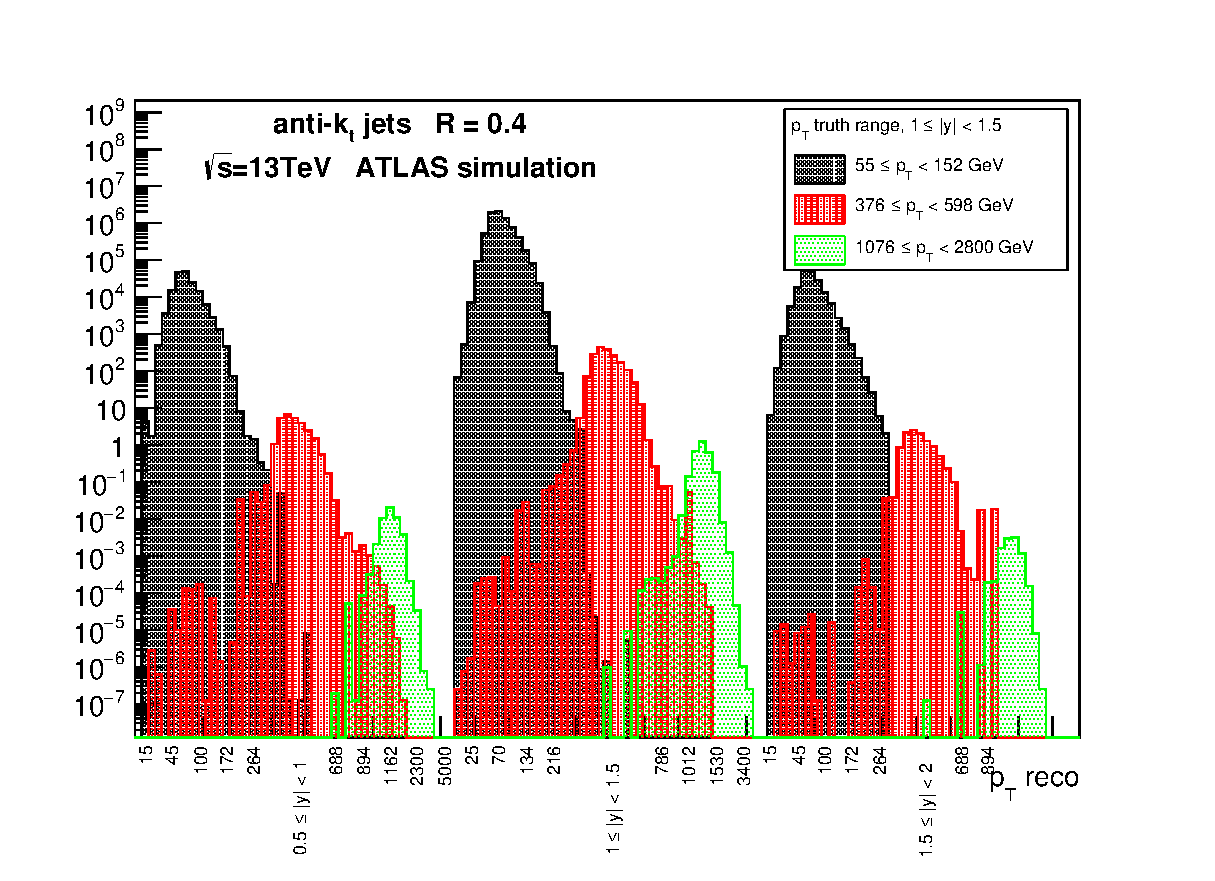
\includegraphics[width=0.49\textwidth]{{Chapter3/UnfoldMatrixSlices22}.eps}
  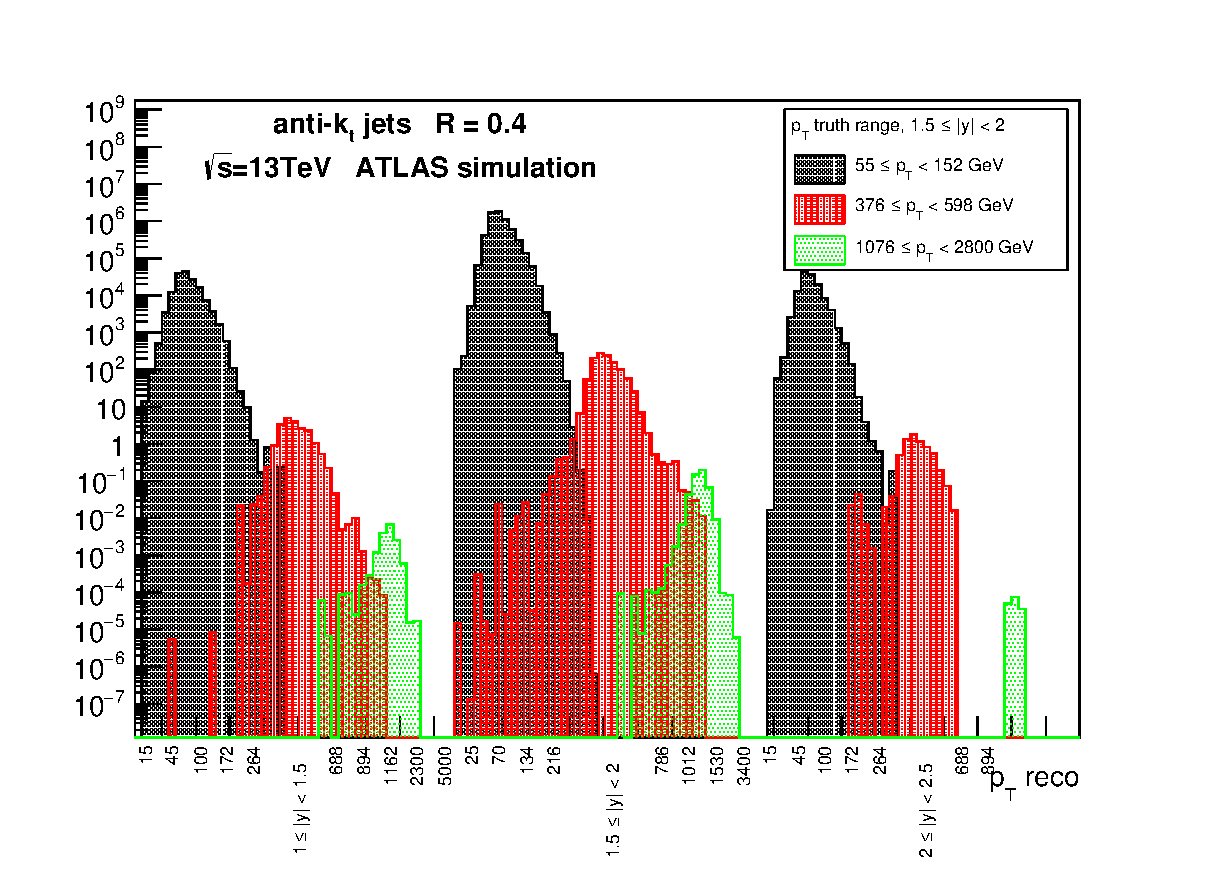
\includegraphics[width=0.49\textwidth]{{Chapter3/UnfoldMatrixSlices33}.eps}
  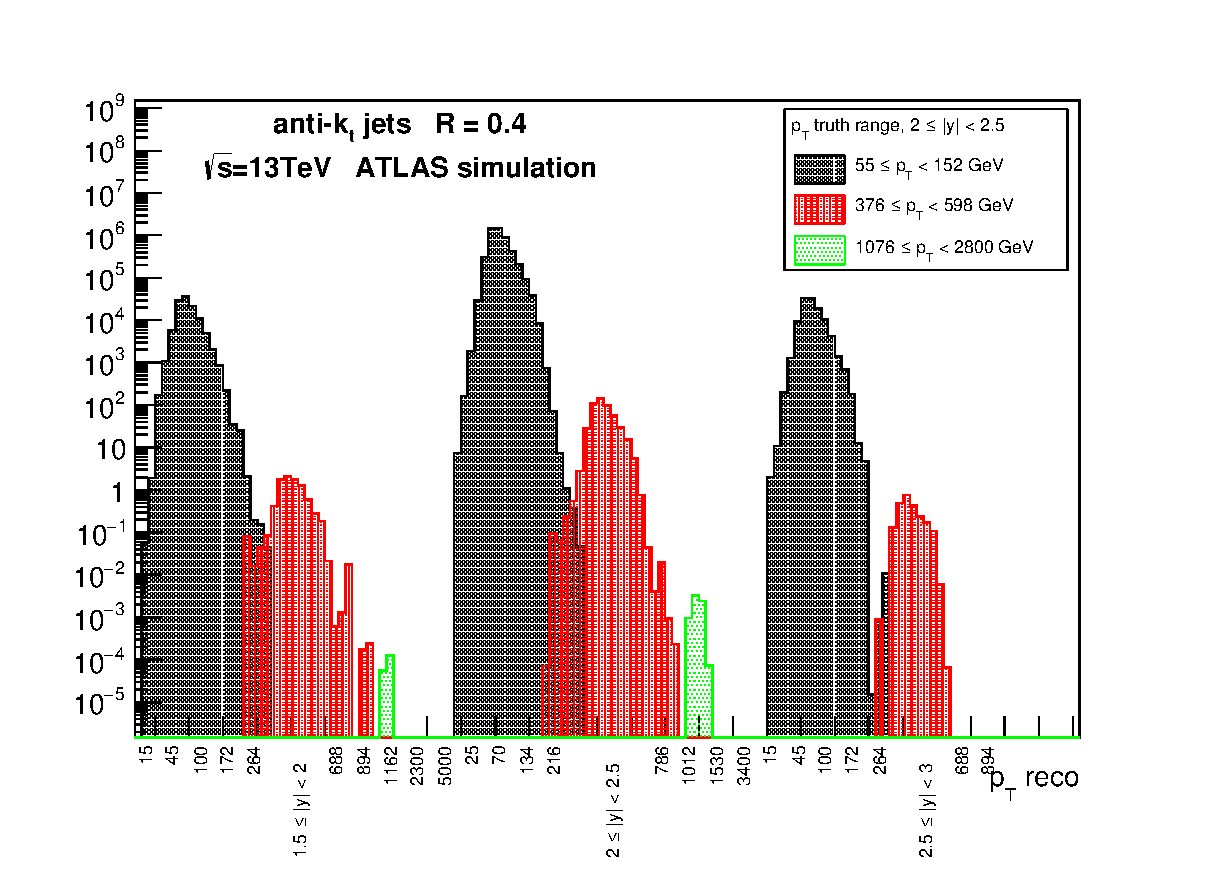
\includegraphics[width=0.49\textwidth]{{Chapter3/UnfoldMatrixSlices44}.eps}
  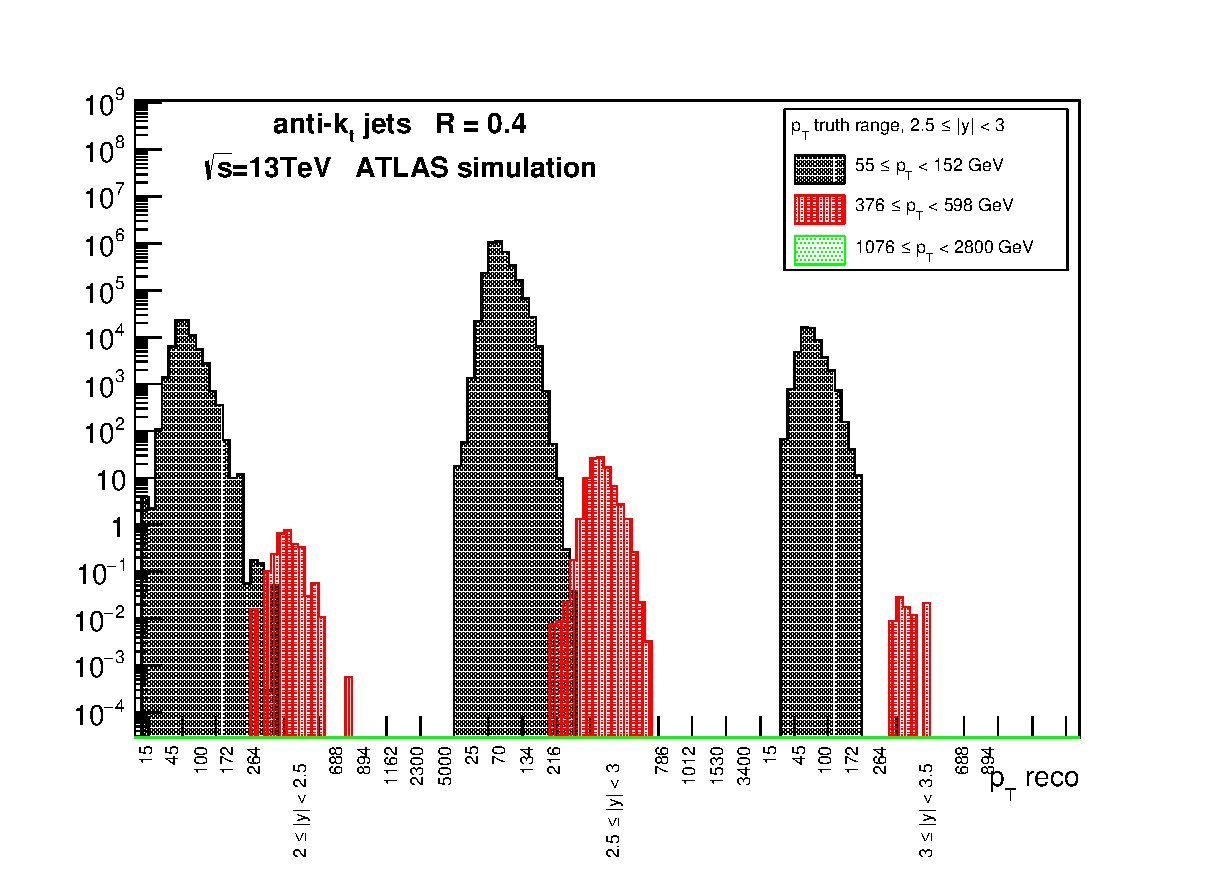
\includegraphics[width=0.49\textwidth]{{Chapter3/UnfoldMatrixSlices55}.eps}
  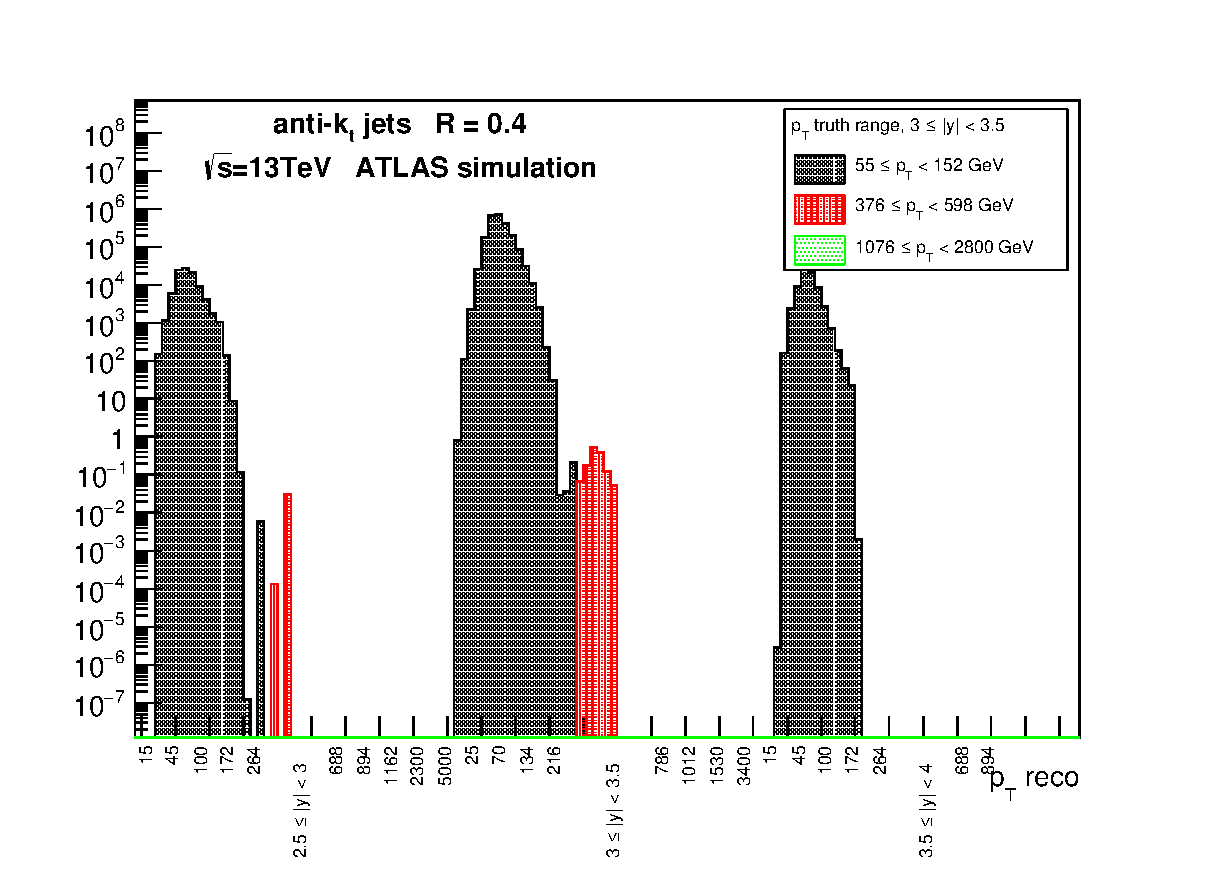
\includegraphics[width=0.49\textwidth]{{Chapter3/UnfoldMatrixSlices66}.eps}
  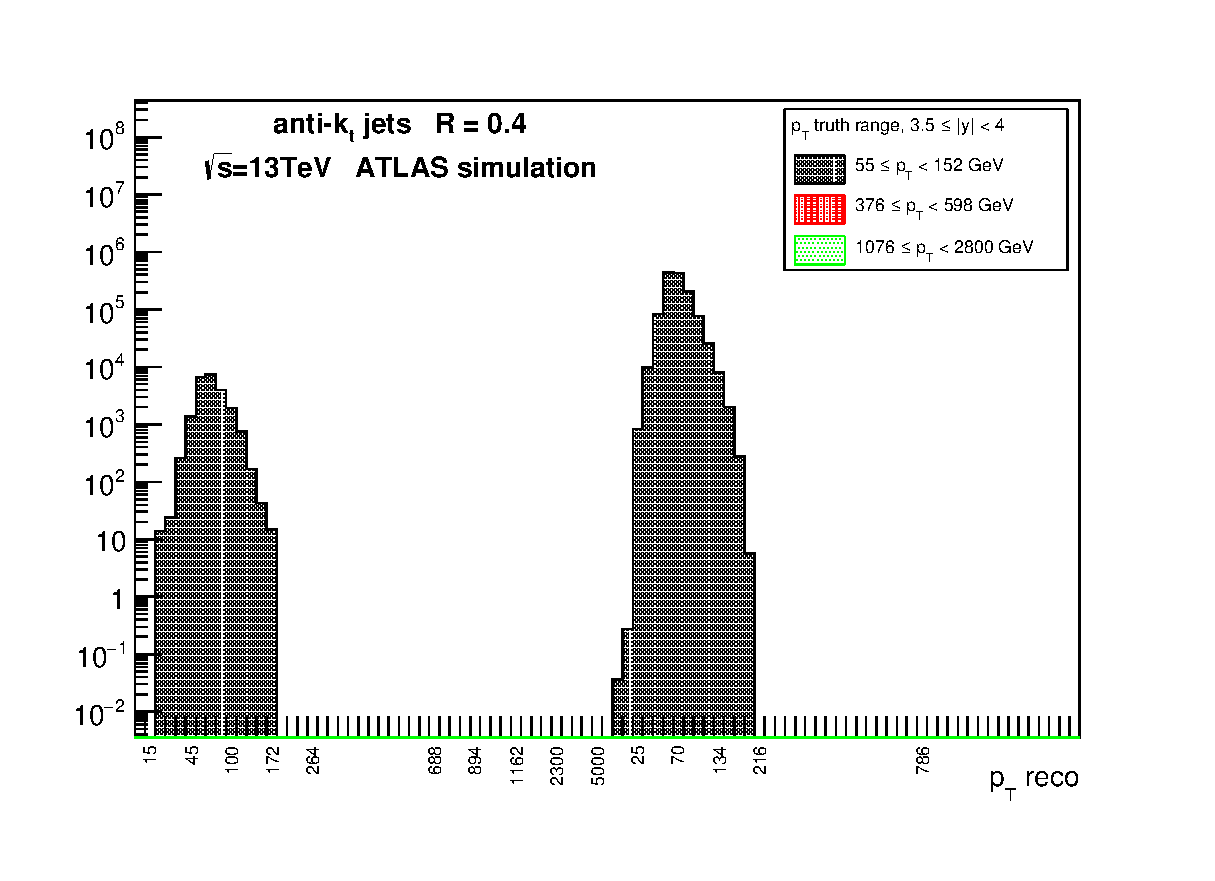
\includegraphics[width=0.49\textwidth]{{Chapter3/UnfoldMatrixSlices77}.eps}
  \caption{Slices in transfer matrix of 2D unfolding method from Figure
    \label{fig:UnfoldingMatrixAll} on $y$-axis represnted by the $\pt$ spectrum
    of reco jets. Slices are done in each rapidity bin for three different ranges
    of $\pt$ of truth jets.}
\end{figure}

\section{Unfolding Results}
\label{sec:UnfoldingResults}

\begin{figure}[H]
  \centering
  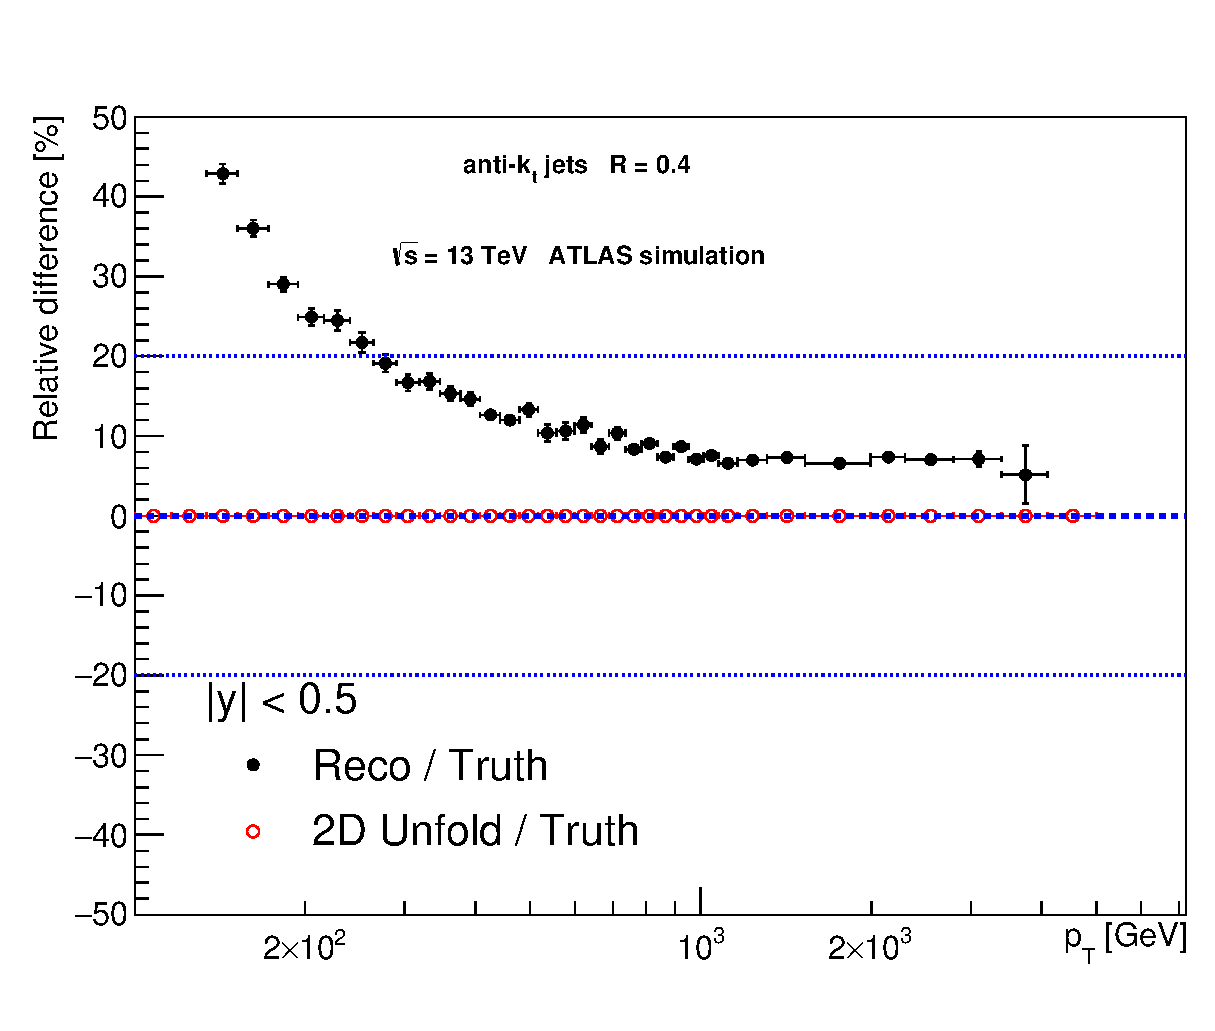
\includegraphics[width=0.49\textwidth]{{Chapter3/SignalUnfolded_VS_Truth0Compare}.eps}
  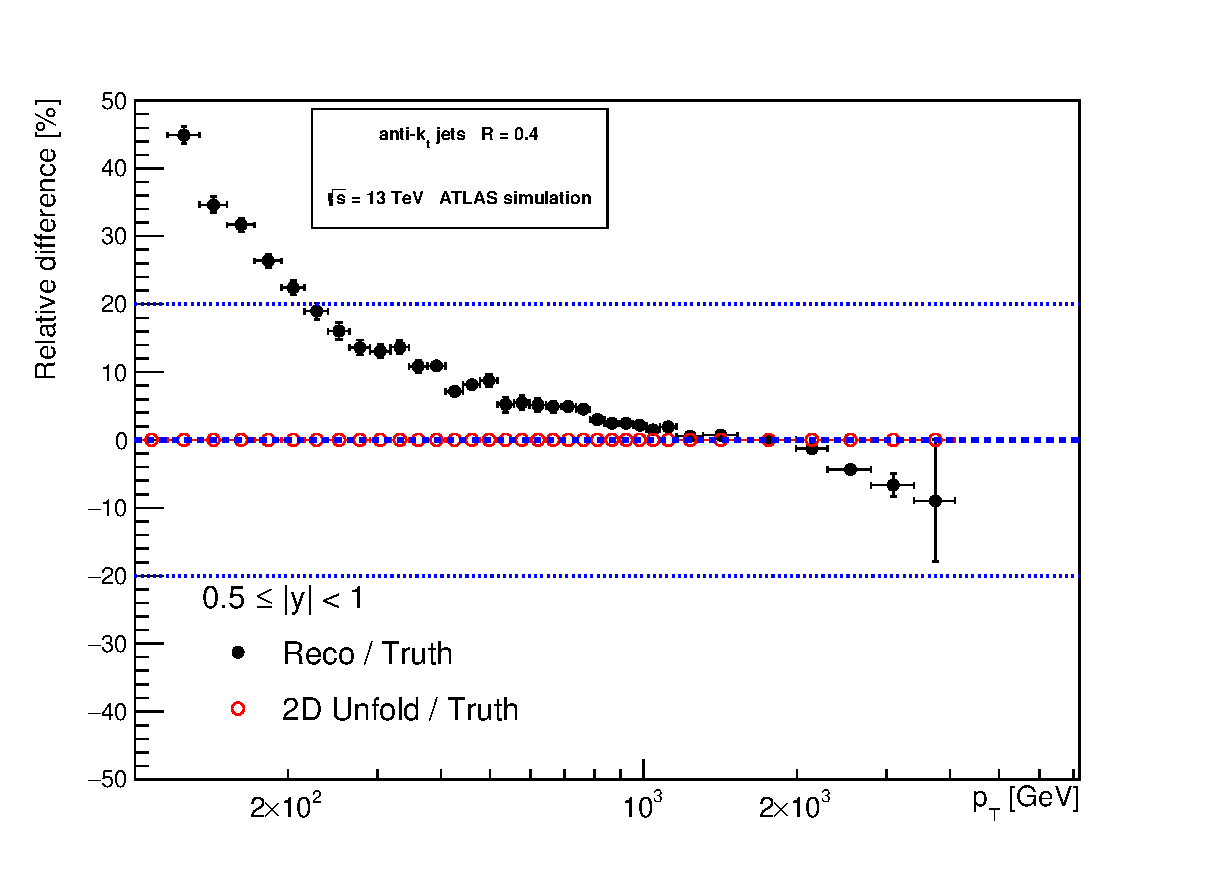
\includegraphics[width=0.49\textwidth]{{Chapter3/SignalUnfolded_VS_Truth1Compare}.eps}
  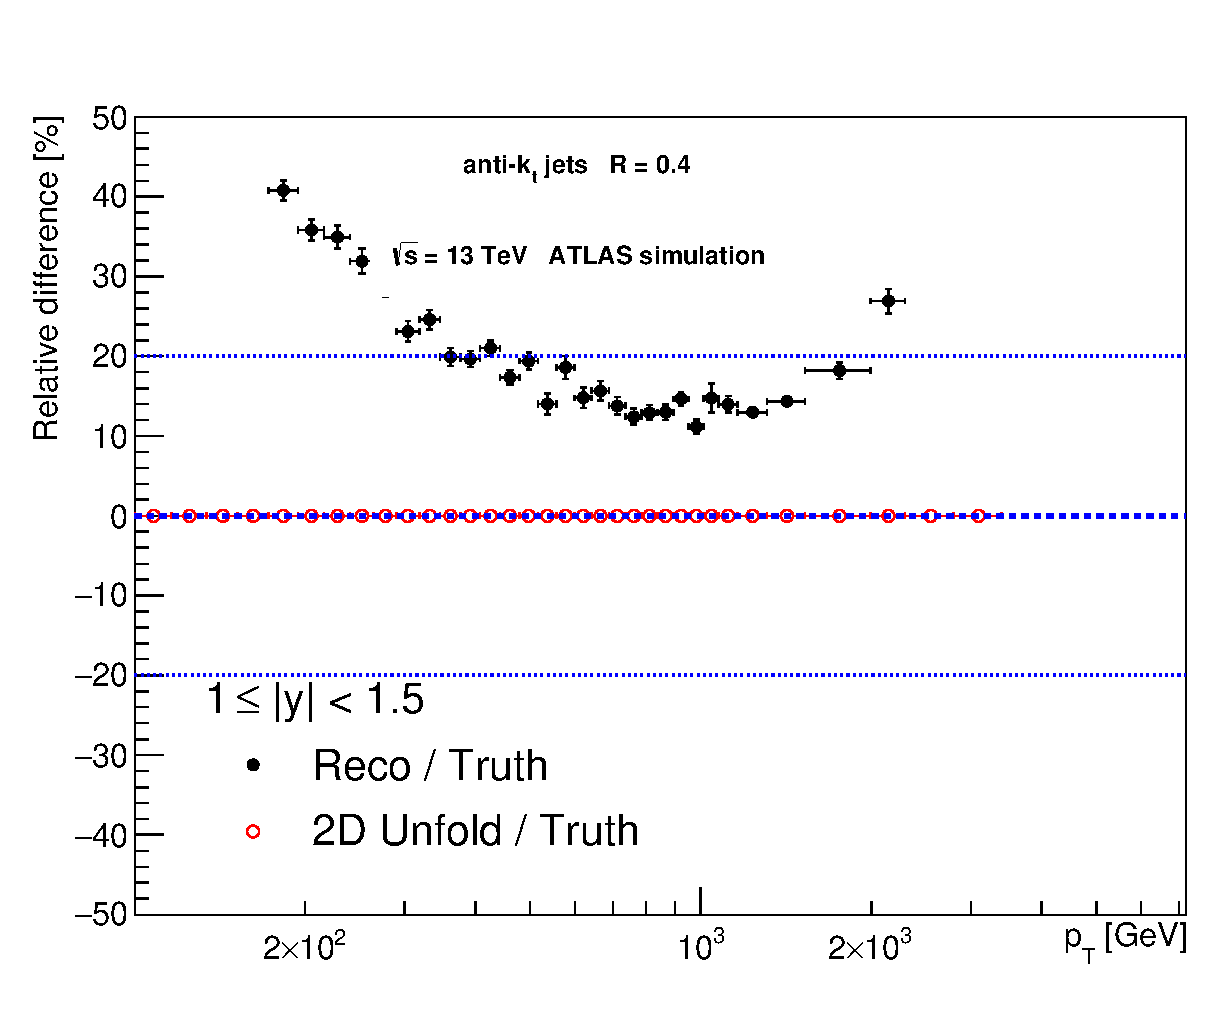
\includegraphics[width=0.49\textwidth]{{Chapter3/SignalUnfolded_VS_Truth2Compare}.eps}
  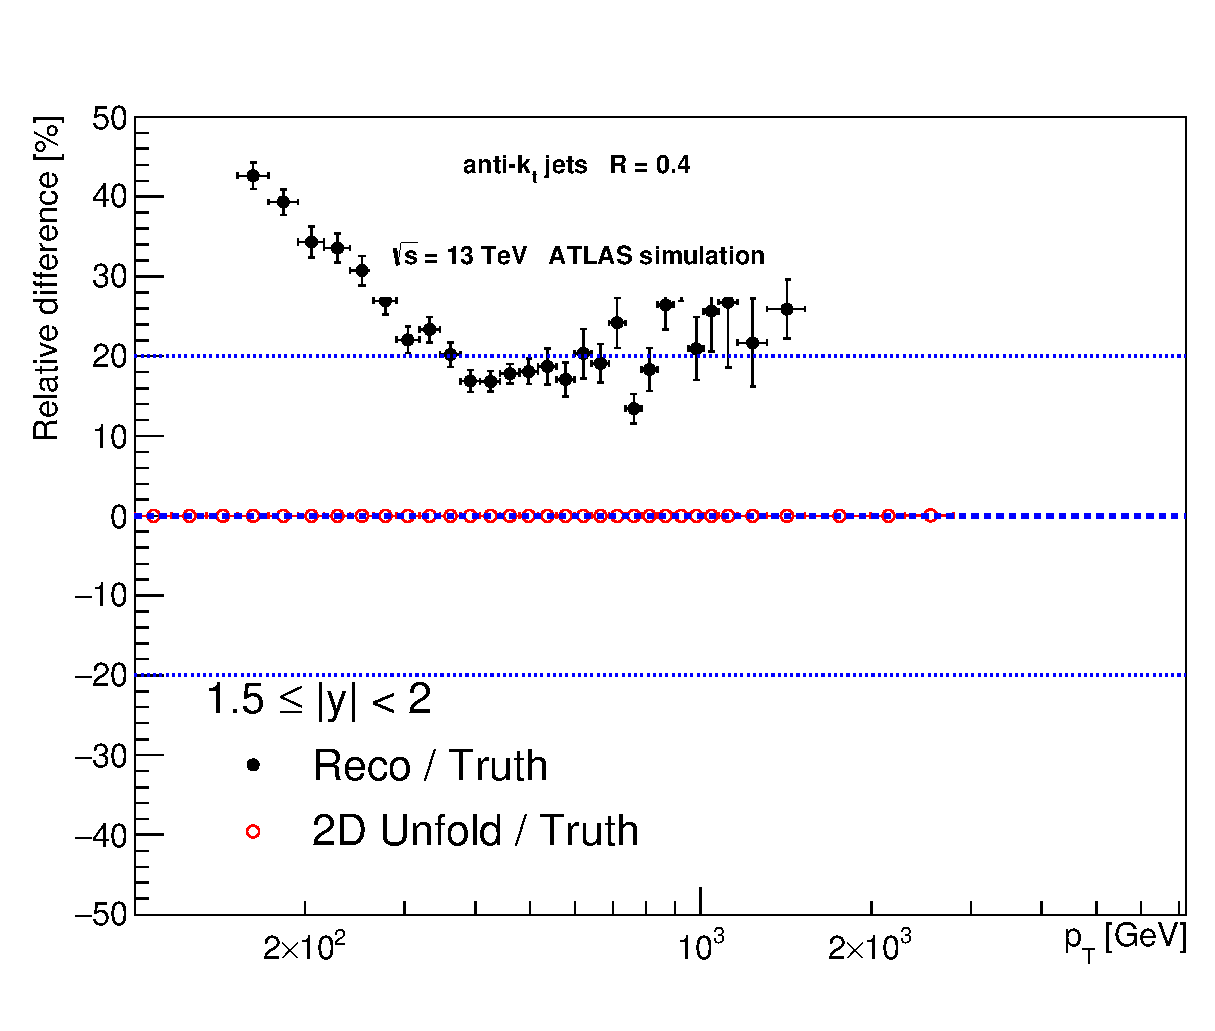
\includegraphics[width=0.49\textwidth]{{Chapter3/SignalUnfolded_VS_Truth3Compare}.eps}
  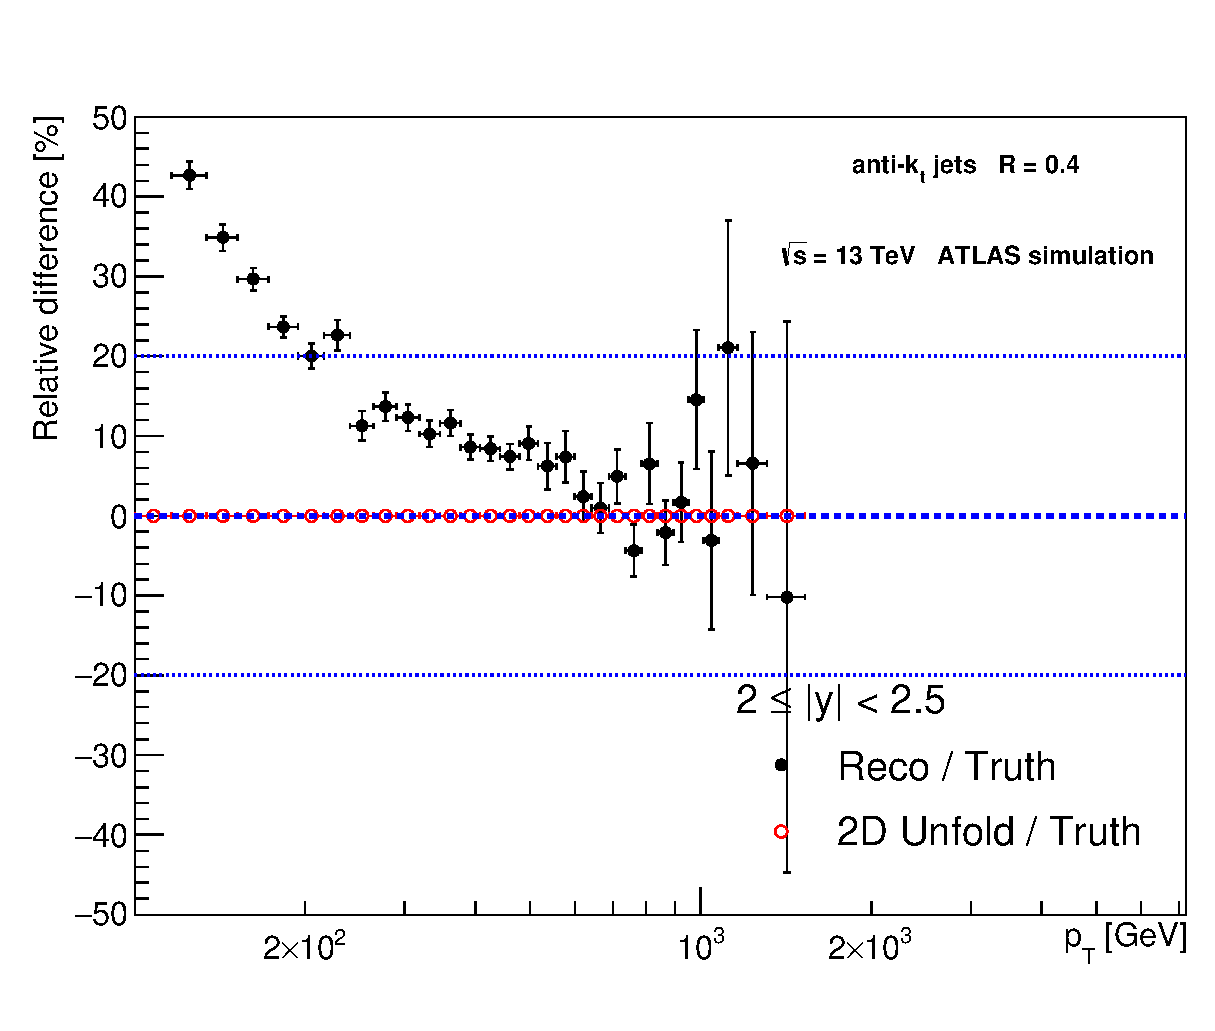
\includegraphics[width=0.49\textwidth]{{Chapter3/SignalUnfolded_VS_Truth4Compare}.eps}
  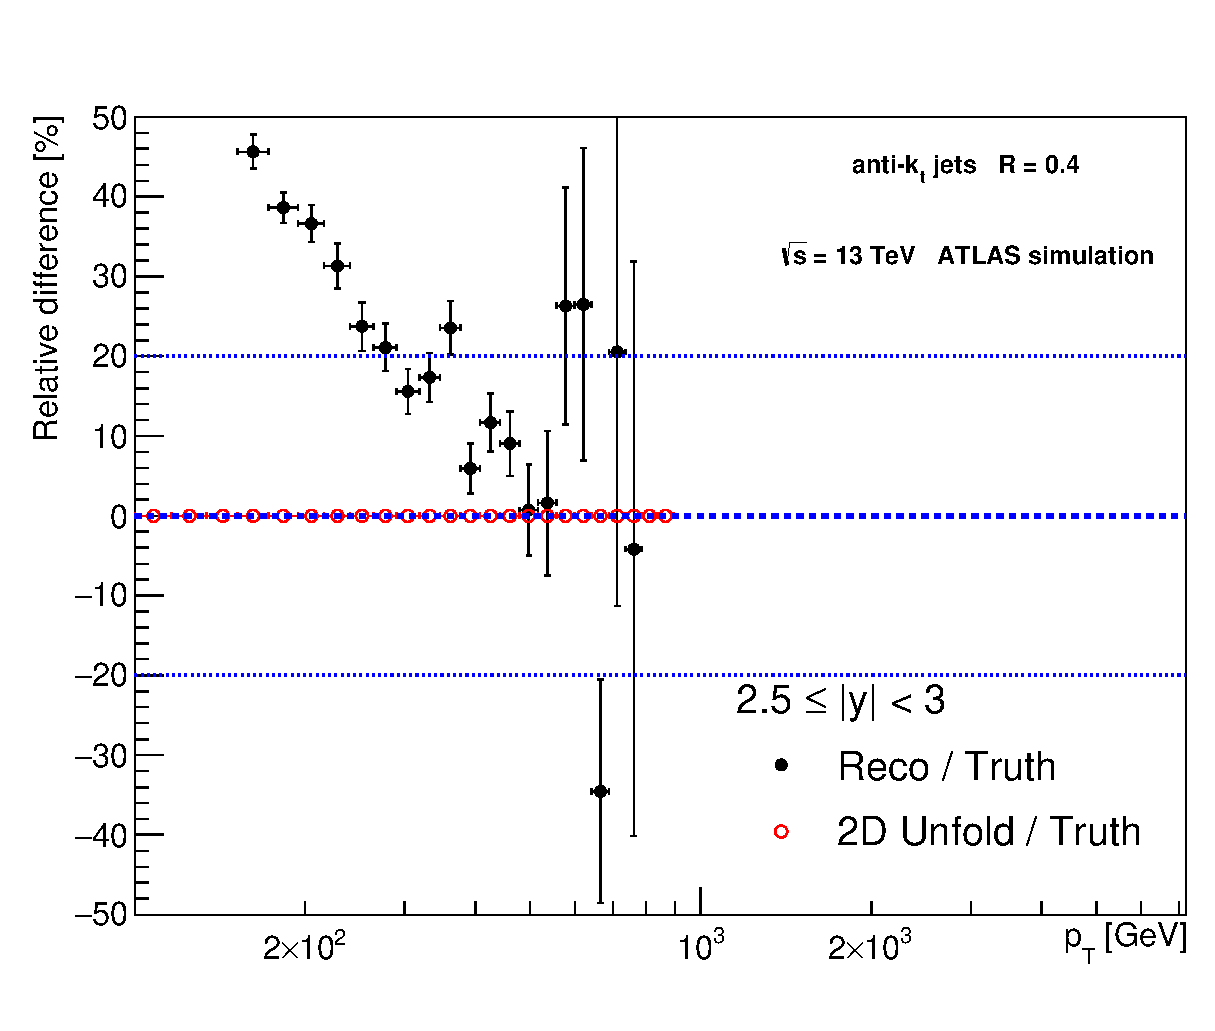
\includegraphics[width=0.49\textwidth]{{Chapter3/SignalUnfolded_VS_Truth5Compare}.eps}
  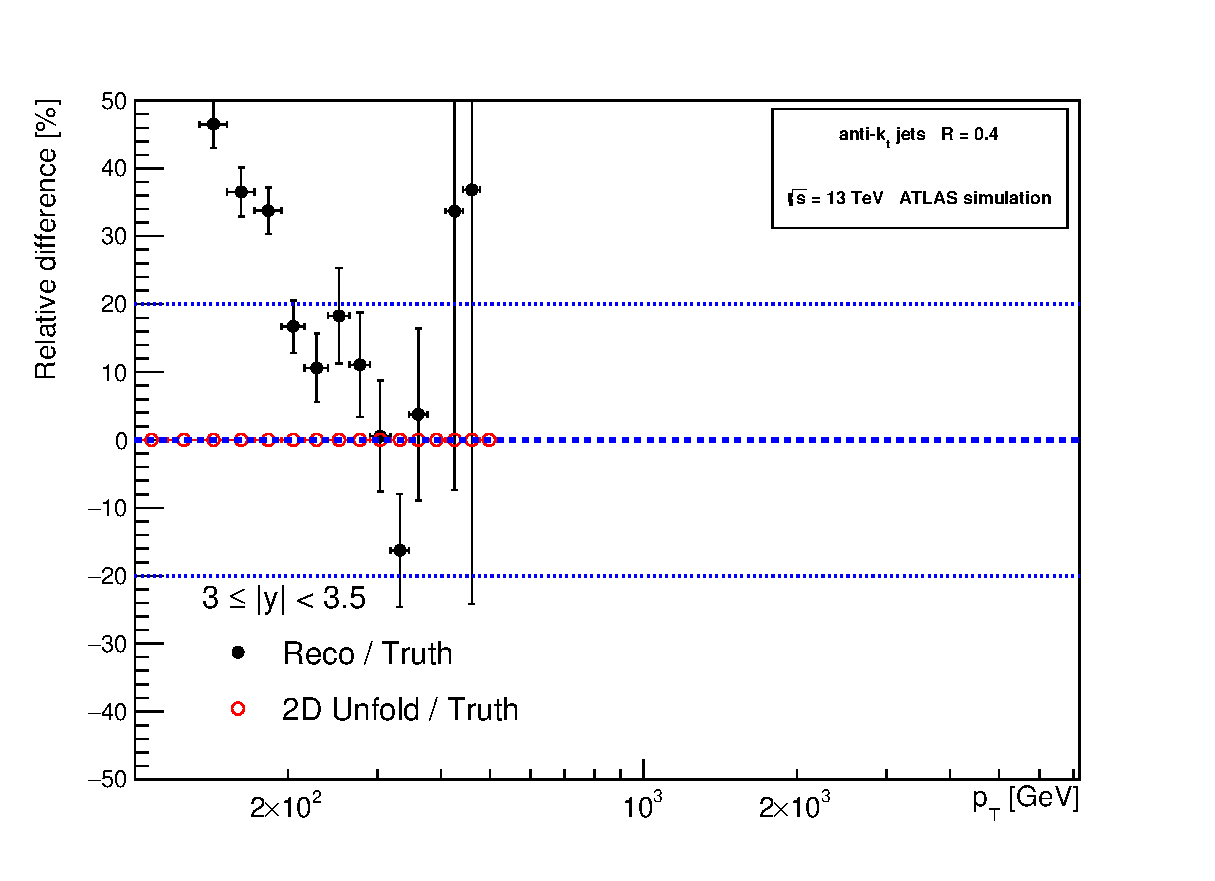
\includegraphics[width=0.49\textwidth]{{Chapter3/SignalUnfolded_VS_Truth6Compare}.eps}
  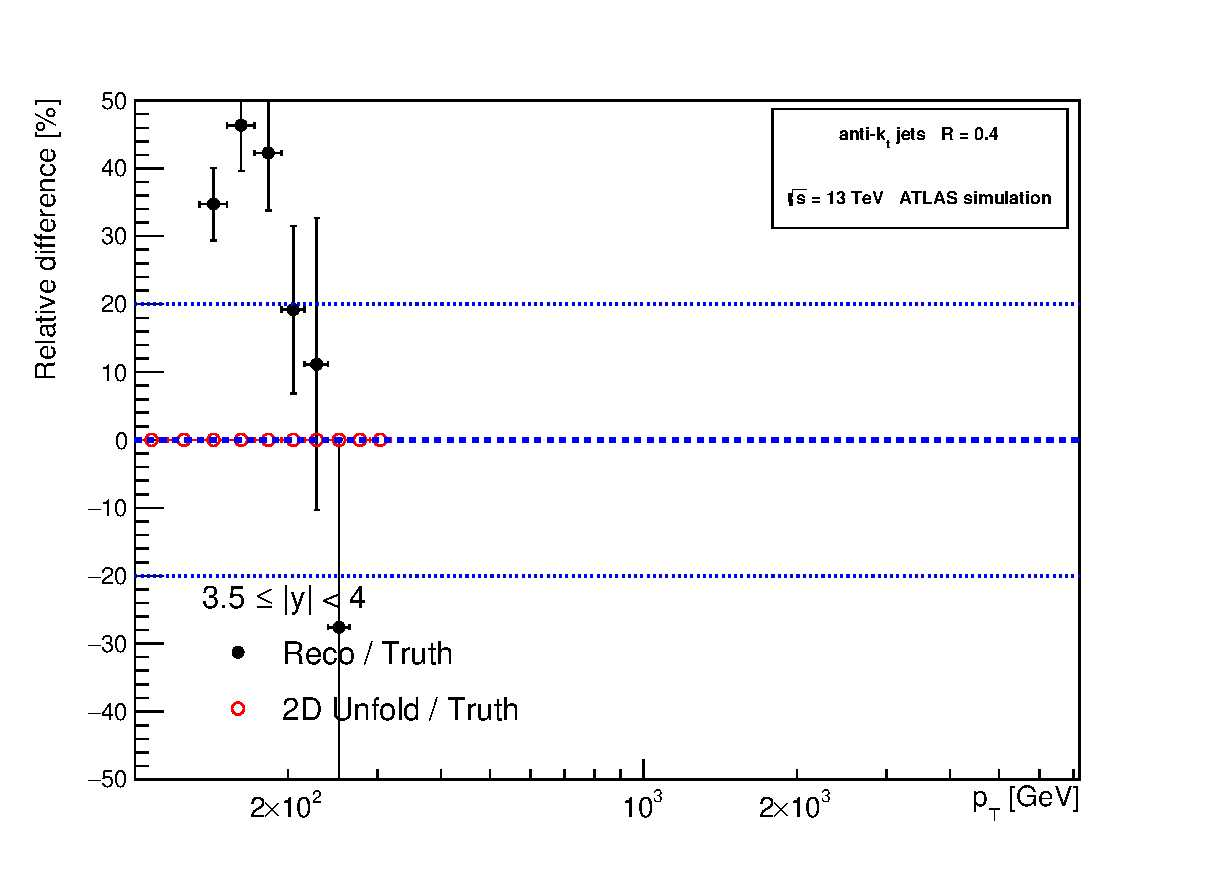
\includegraphics[width=0.49\textwidth]{{Chapter3/SignalUnfolded_VS_Truth7Compare}.eps}
  \caption{Comparison of $\pt$ spectra of reco jets and the unfolded $\pt$
  spectra (2D unfolding) with the $\pt$ spectra of the truth jets for 8
  different rapidity bins.}
\end{figure}

\section{Simple and 2D Unfolding}
\label{sec:SimpleAnd2DUnfolding}

\begin{figure}[H]
  \centering
  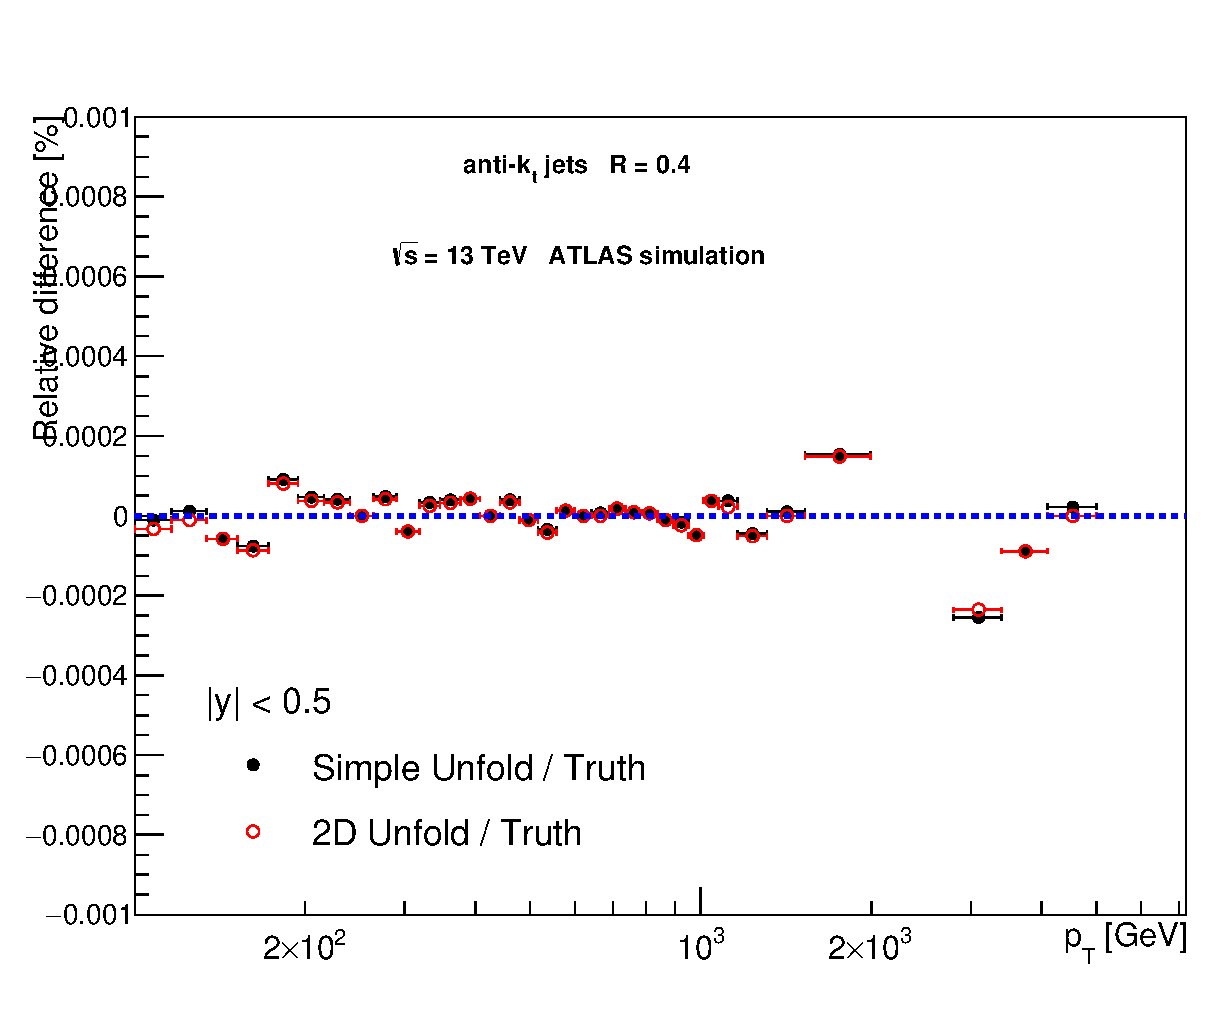
\includegraphics[width=0.49\textwidth]{{Chapter3/UnfoldedSimpleComplex_VS_Truth0Compare}.eps}
  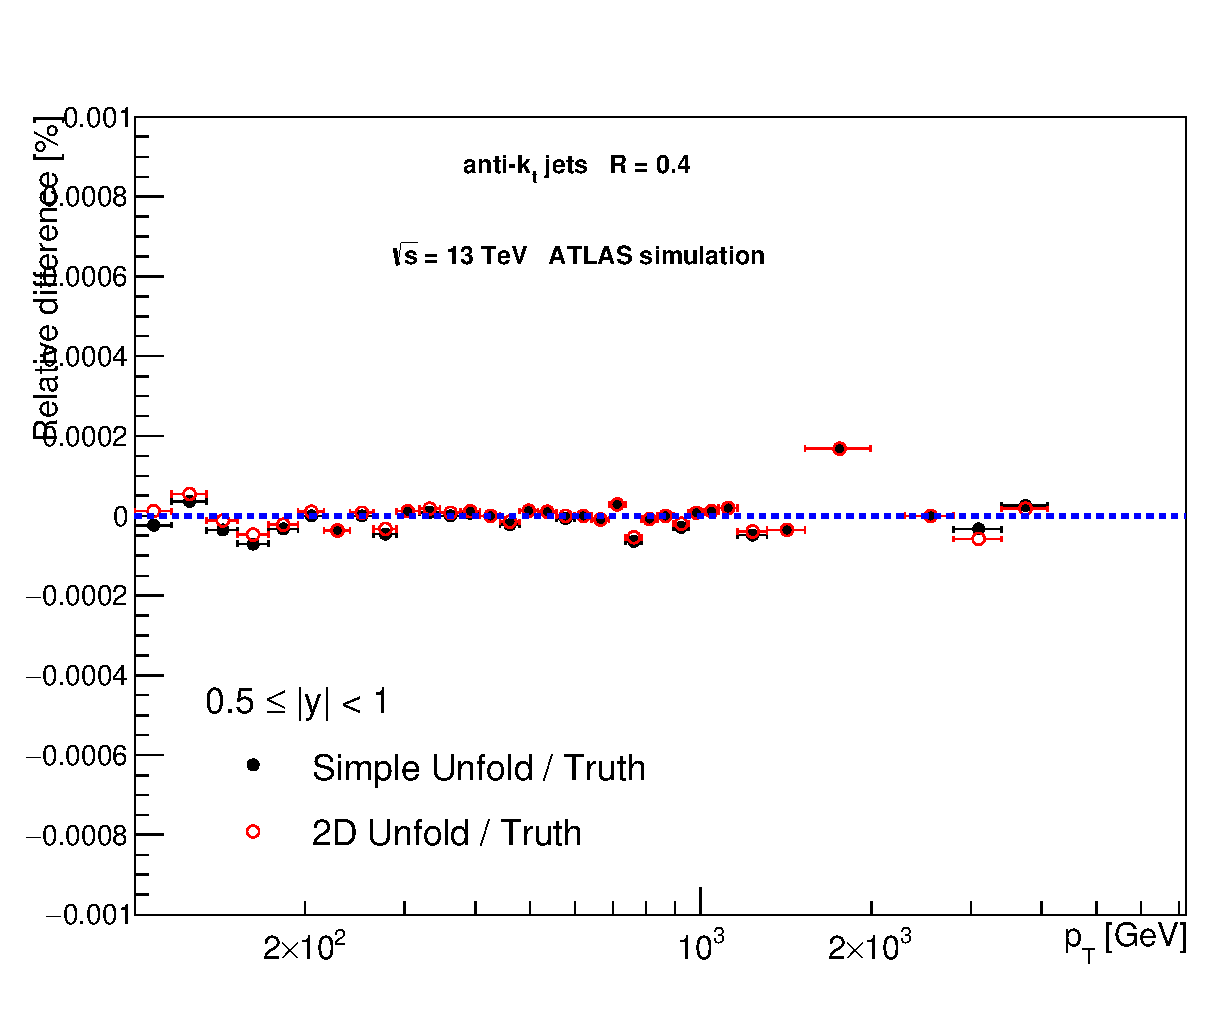
\includegraphics[width=0.49\textwidth]{{Chapter3/UnfoldedSimpleComplex_VS_Truth1Compare}.eps}
  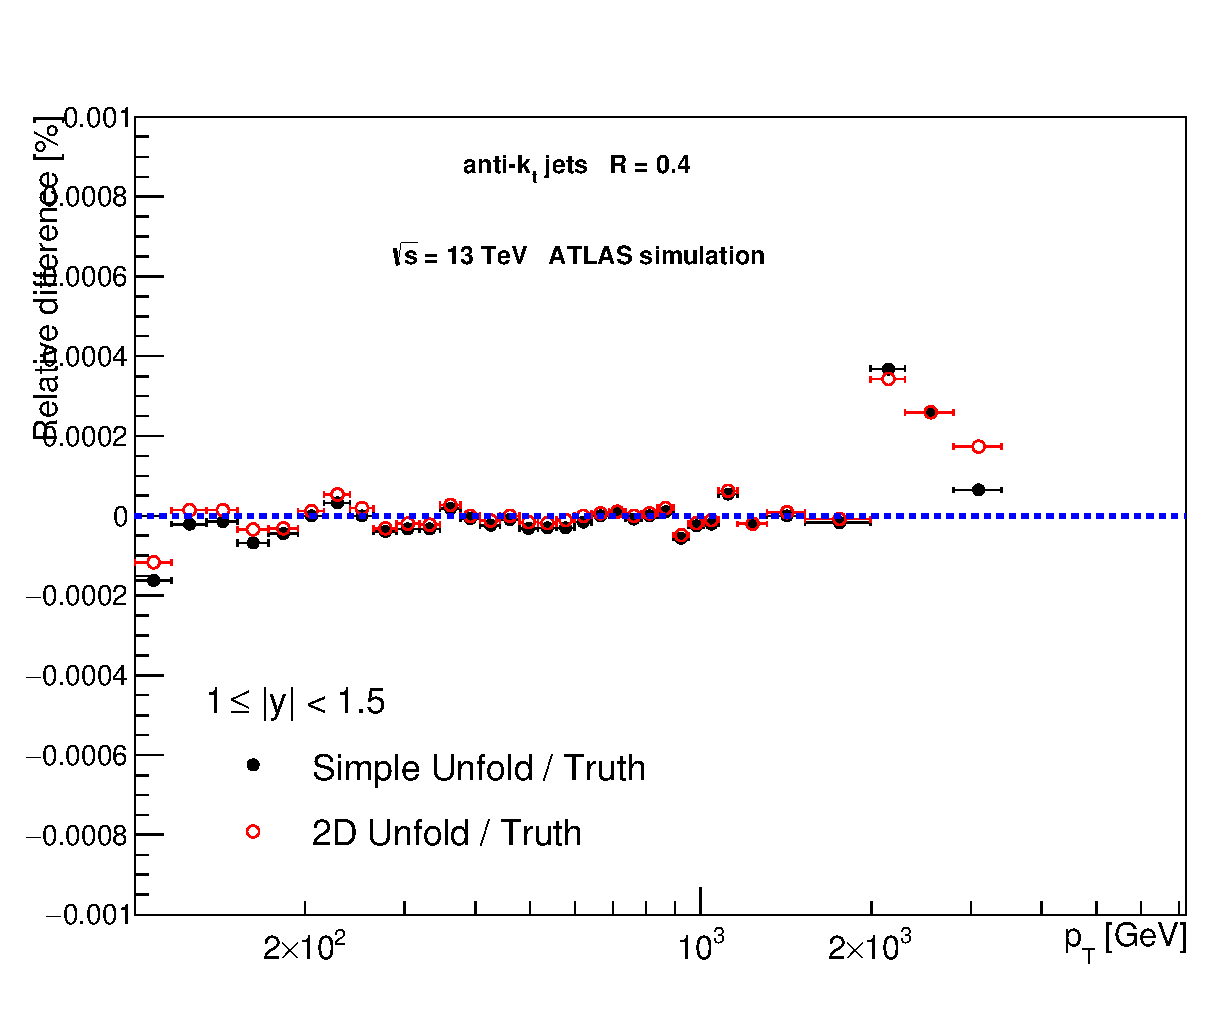
\includegraphics[width=0.49\textwidth]{{Chapter3/UnfoldedSimpleComplex_VS_Truth2Compare}.eps}
  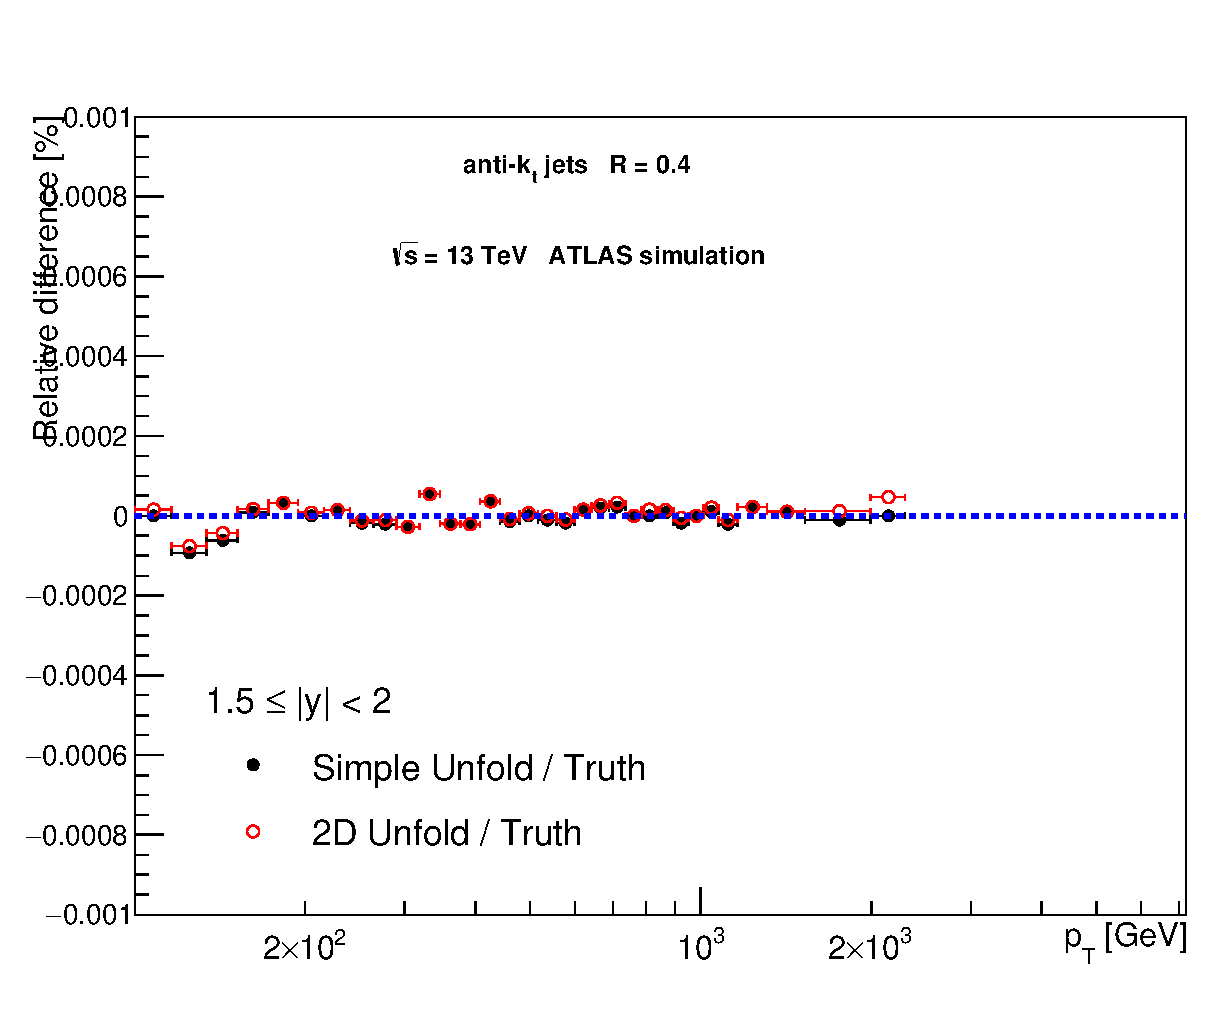
\includegraphics[width=0.49\textwidth]{{Chapter3/UnfoldedSimpleComplex_VS_Truth3Compare}.eps}
  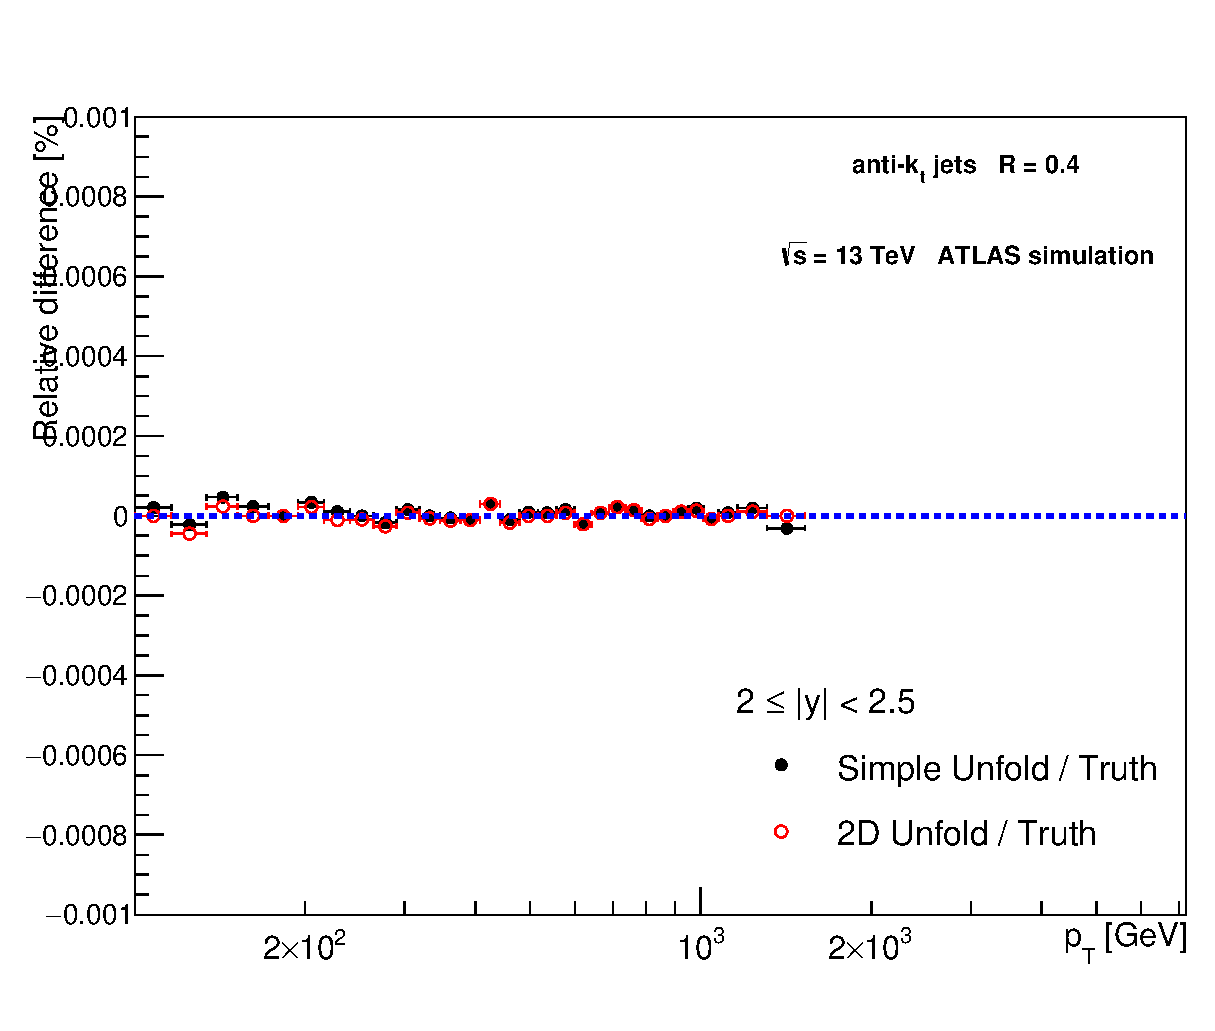
\includegraphics[width=0.49\textwidth]{{Chapter3/UnfoldedSimpleComplex_VS_Truth4Compare}.eps}
  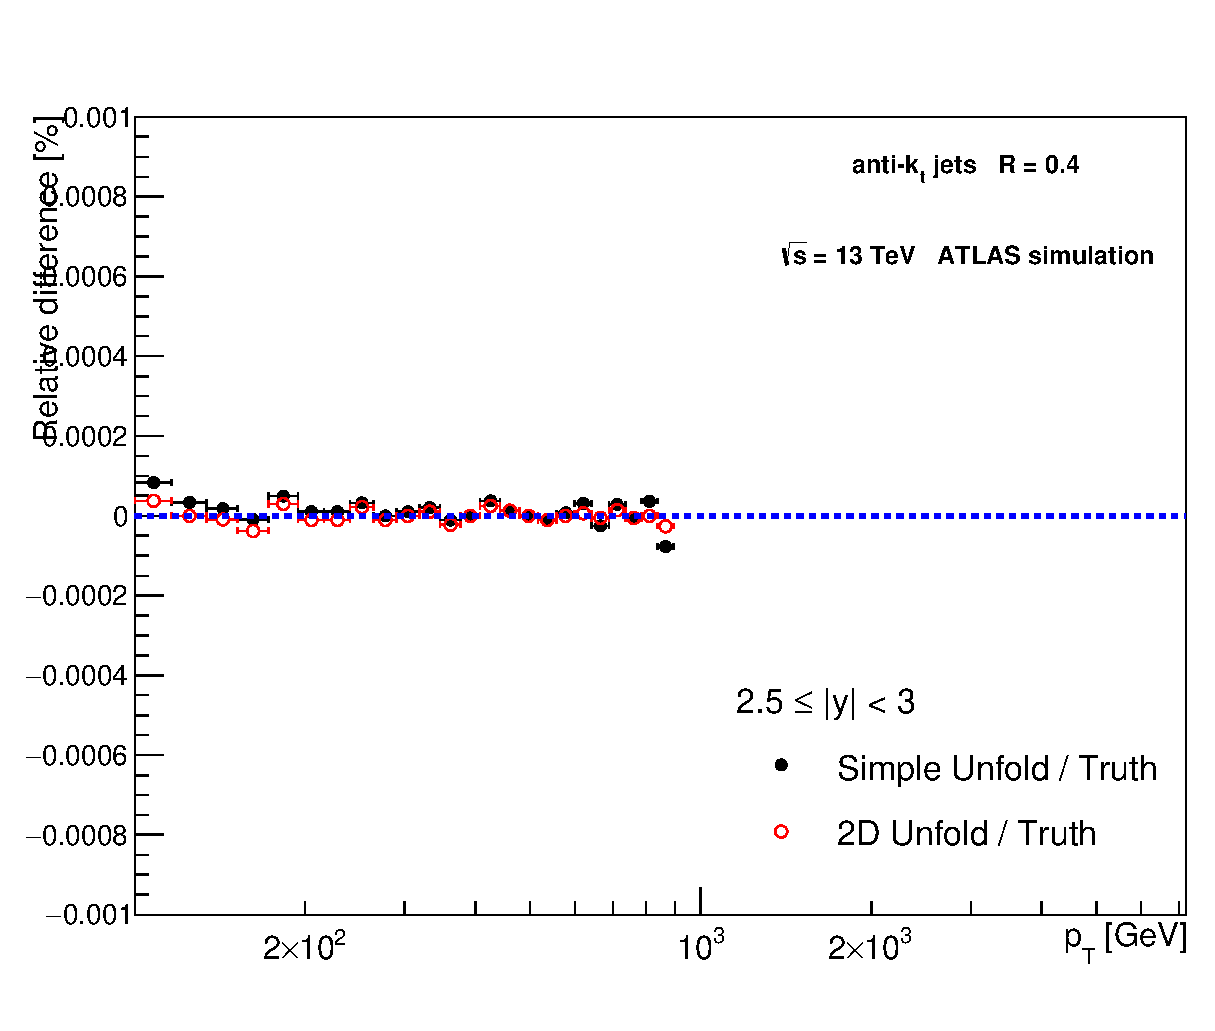
\includegraphics[width=0.49\textwidth]{{Chapter3/UnfoldedSimpleComplex_VS_Truth5Compare}.eps}
  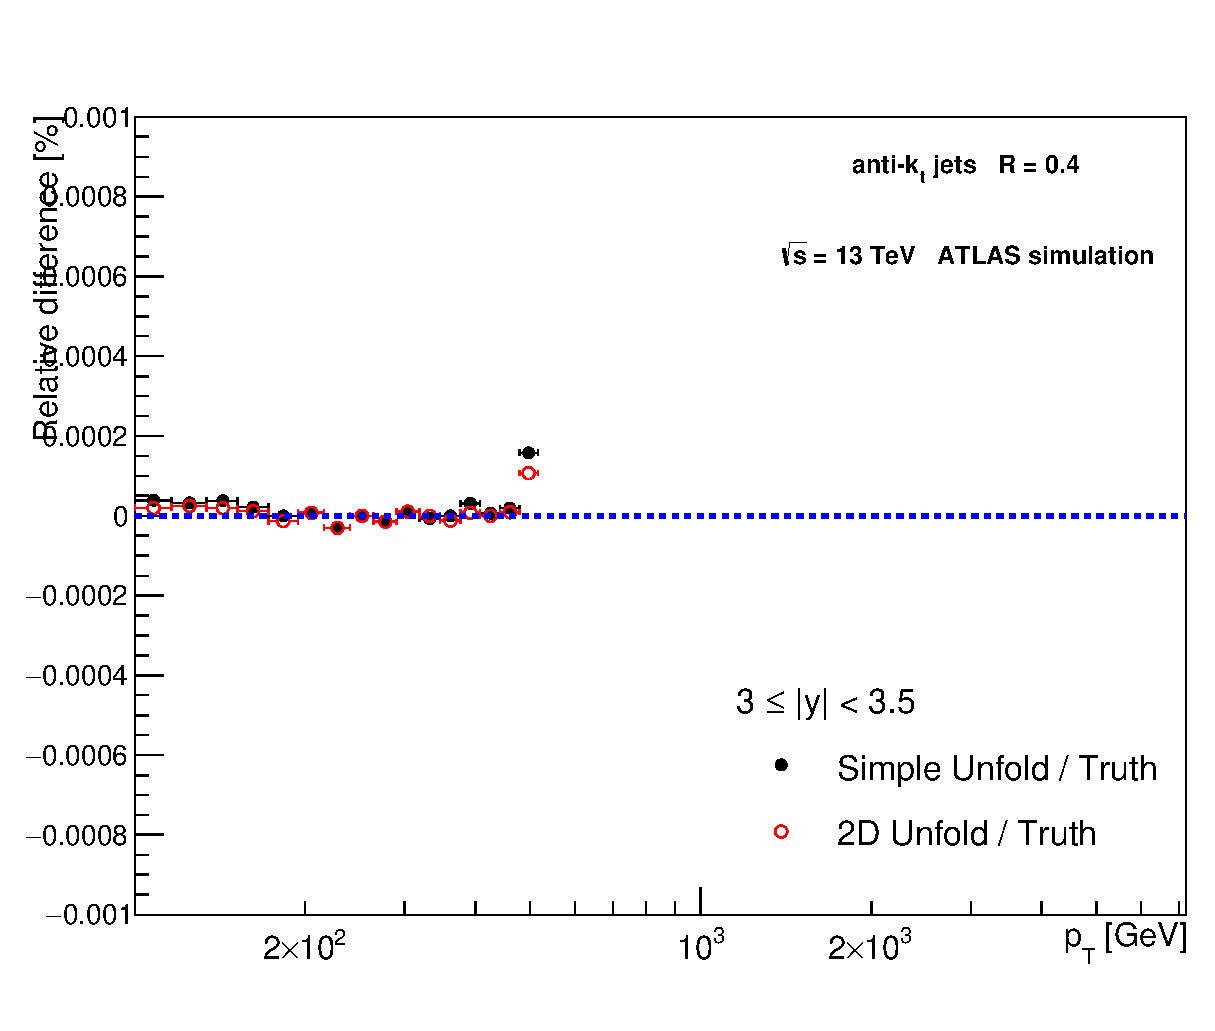
\includegraphics[width=0.49\textwidth]{{Chapter3/UnfoldedSimpleComplex_VS_Truth6Compare}.eps}
  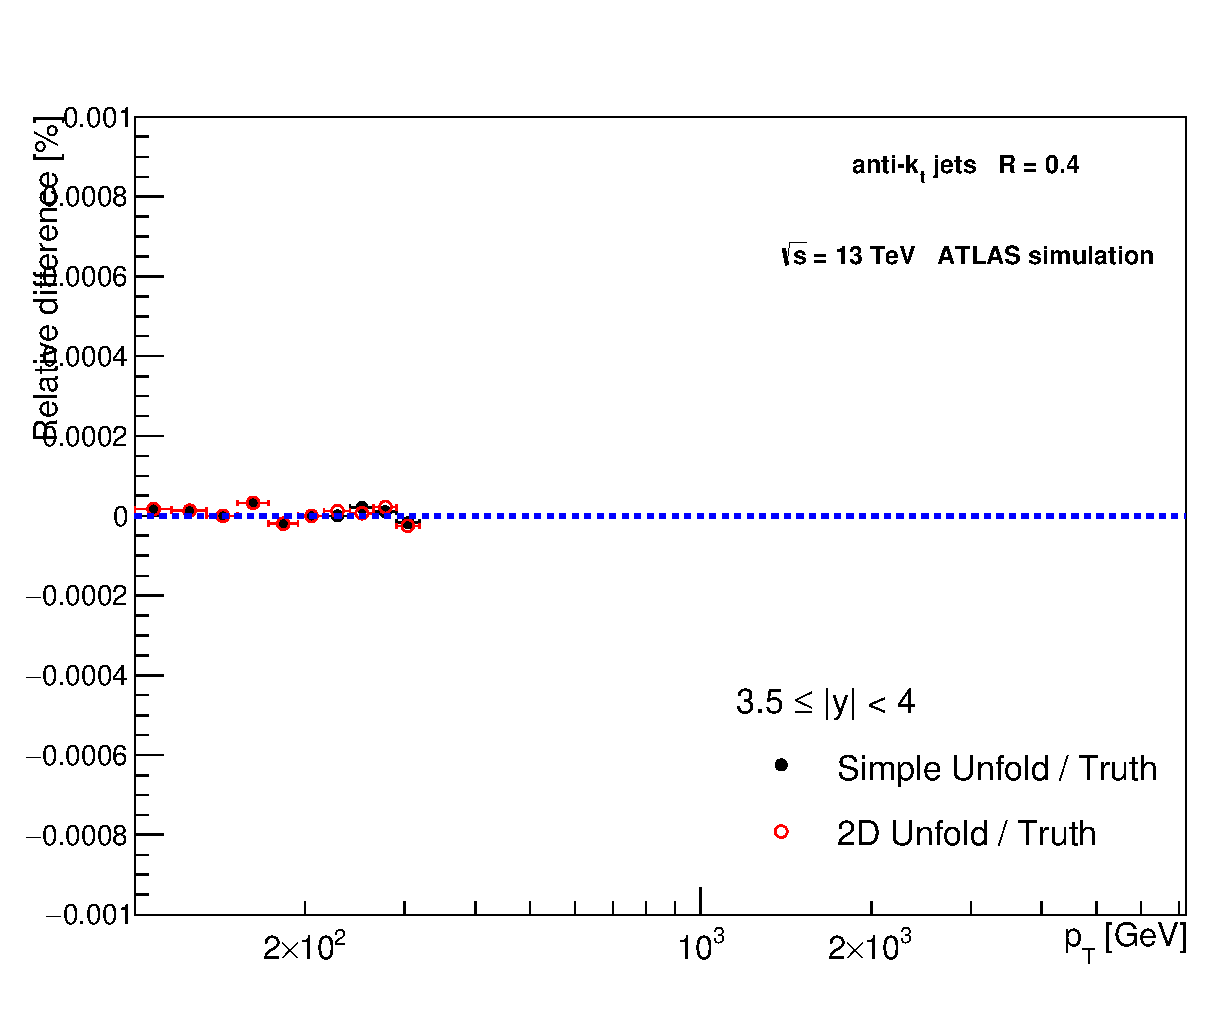
\includegraphics[width=0.49\textwidth]{{Chapter3/UnfoldedSimpleComplex_VS_Truth7Compare}.eps}
  \caption{Comparison of results obtained by two unfolding method - simple and
    2D unfolding - with the $\pt$ spectra of truth jets for 8 different
    rapidity bins.}
\end{figure}

\chapter{NLO QCD Prediction}
\label{App:UnfoldingAndPrediction}

\newpage

\section{Predictions for Run I and Run II}
\label{sec:PredictionsForRunIAndII}

\begin{figure}[H]
  \centering
  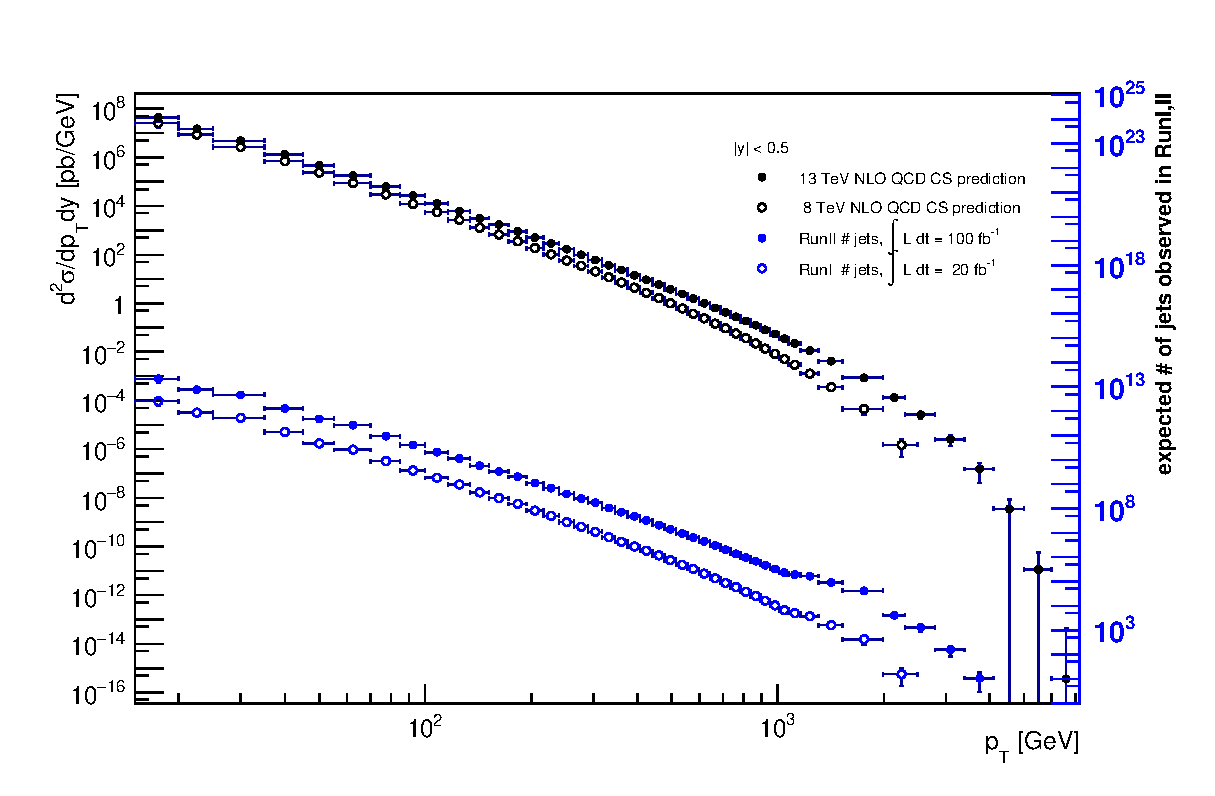
\includegraphics[width=0.9\textwidth]{{Chapter3/PredictionCompare0}.eps}
  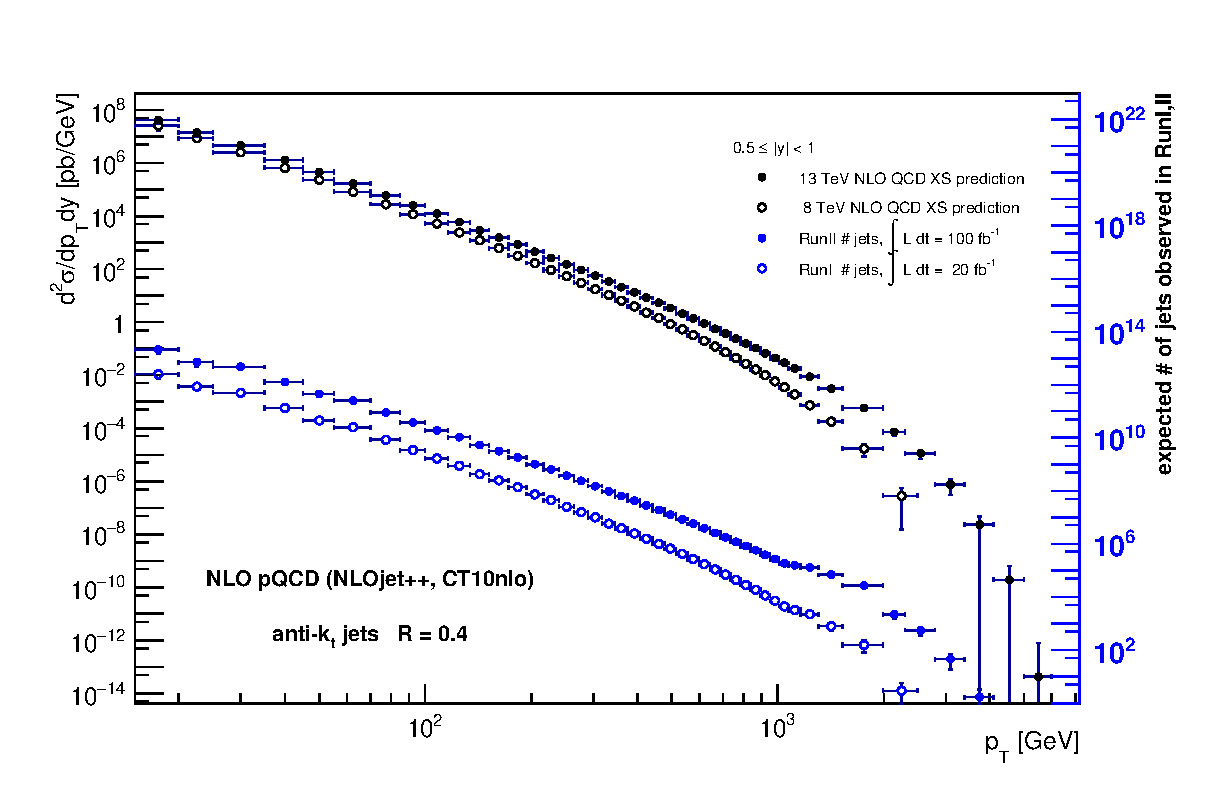
\includegraphics[width=0.9\textwidth]{{Chapter3/PredictionCompare1}.eps}
  \caption{Comparison of NLO QCD prediction of double differential inclusive jet
    cross section (black) in $\pt$ and rapidity of $pp$ collisions at $\rts=13\TeV$
    (filled circles) corresponding to LHC Run II and $\rts=8\TeV$ (empty circles)
    corresponding to LHC Run I. The cross section is multiplied by integrated
    luminosities and $\pt$ bin width to obtain expected number of jets observed in
    each $\pt$ bin (blue). Figures show the comparison for $0.5<|y|$ (top) and
    $0.5\leq|y|<1$ (bottom) rapidity bins.}
\end{figure}

\begin{figure}[p]
  \centering
  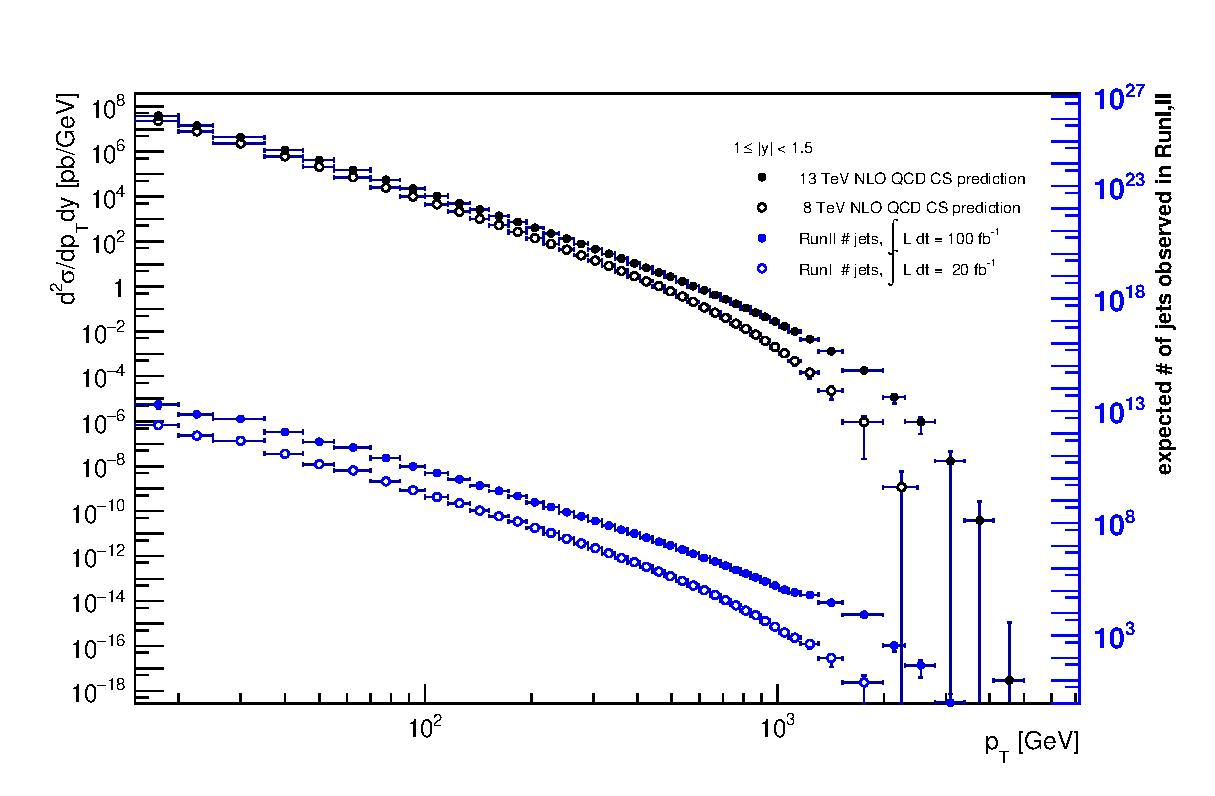
\includegraphics[width=0.9\textwidth]{{Chapter3/PredictionCompare2}.eps}
  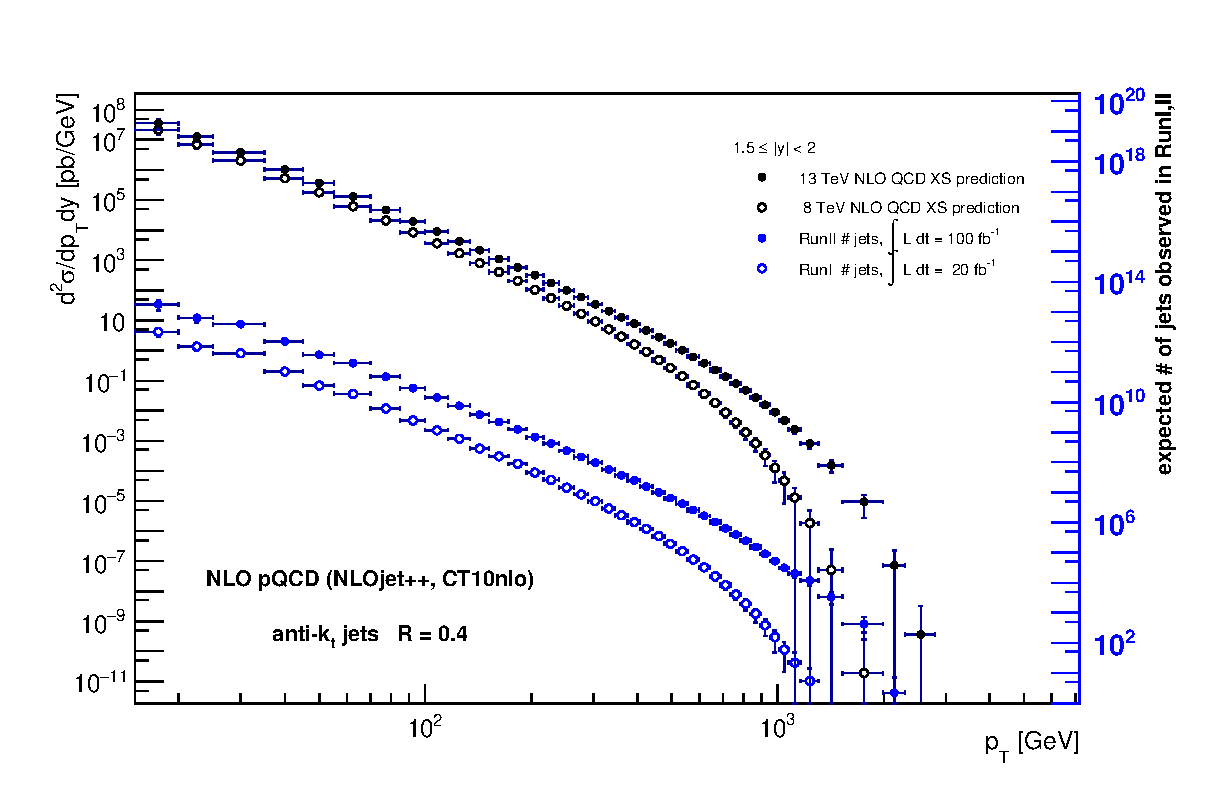
\includegraphics[width=0.9\textwidth]{{Chapter3/PredictionCompare3}.eps}
  \caption{Comparison of NLO QCD prediction of double differential inclusive jet
    cross section (black) in $\pt$ and rapidity of $pp$ collisions at $\rts=13\TeV$
    (filled circles) corresponding to LHC Run II and $\rts=8\TeV$ (empty circles)
    corresponding to LHC Run I. The cross section is multiplied by integrated
    luminosities and $\pt$ bin width to obtain expected number of jets observed in
    each $\pt$ bin (blue). Figures show the comparison for $1\leq|y|<1.5$ (top) and $1.5
    \leq |y| < 2$ (bottom) rapidity bins.}
\end{figure}

\begin{figure}[p]
  \centering
  \includegraphics[width=0.9\textwidth]{{Chapter3/PredictionCompare4}.eps}
  \includegraphics[width=0.9\textwidth]{{Chapter3/PredictionCompare5}.eps}
  \caption{Comparison of NLO QCD prediction of double differential inclusive jet
    cross section (black) in $\pt$ and rapidity of $pp$ collisions at $\rts=13\TeV$
    (filled circles) corresponding to LHC Run II and $\rts=8\TeV$ (empty circles)
    corresponding to LHC Run I. The cross section is multiplied by integrated
    luminosities and $\pt$ bin width to obtain expected number of jets observed in
    each $\pt$ bin (blue). Figures show the comparison for $2\leq|y|<2.5$ (top) and $2.5
    \leq |y| < 3$ (bottom) rapidity bins.}
\end{figure}

\section{NLO Uncertainties}
\label{sec:NLOUncertainties}

\begin{figure}[H]
  \centering
  \includegraphics[width=0.49\textwidth]{{Chapter3/NLO_Systematics8_TeV0}.eps}
  \includegraphics[width=0.49\textwidth]{{Chapter3/NLO_Systematics13_TeV0}.eps}
  \includegraphics[width=0.49\textwidth]{{Chapter3/NLO_Systematics8_TeV1}.eps}
  \includegraphics[width=0.49\textwidth]{{Chapter3/NLO_Systematics13_TeV1}.eps}
  \includegraphics[width=0.49\textwidth]{{Chapter3/NLO_Systematics8_TeV2}.eps}
  \includegraphics[width=0.49\textwidth]{{Chapter3/NLO_Systematics13_TeV2}.eps}
  \caption{NLO uncertainties for NLO QCD predictions of inclusive jet double
    differential cross section of $pp$ collisions at $\rts=8\TeV$ (left) and
    $\rts=13\TeV$ (right) for $|y|<0.5$ (top), $0.5\leq|y|<1$ (middle) and
    $1\leq|y|<1.5$ (bottom) rapidity bins.}
\end{figure}

\begin{figure}[p]
  \centering
  \includegraphics[width=0.49\textwidth]{{Chapter3/NLO_Systematics8_TeV3}.eps}
  \includegraphics[width=0.49\textwidth]{{Chapter3/NLO_Systematics13_TeV3}.eps}
  \includegraphics[width=0.49\textwidth]{{Chapter3/NLO_Systematics8_TeV4}.eps}
  \includegraphics[width=0.49\textwidth]{{Chapter3/NLO_Systematics13_TeV4}.eps}
  \includegraphics[width=0.49\textwidth]{{Chapter3/NLO_Systematics8_TeV5}.eps}
  \includegraphics[width=0.49\textwidth]{{Chapter3/NLO_Systematics13_TeV5}.eps}
  \caption{NLO uncertainties for NLO QCD predictions of inclusive jet double
    differential cross section of $pp$ collisions at $\rts=8\TeV$ (left) and
    $\rts=13\TeV$ (right) for $1.5\leq|y|<2$ (top), $2\leq|y|<2.5$ (middle) and
    $2.5\leq|y|<3$ (bottom) rapidity bins.}
\end{figure}

\section{Pythia and NLO}
\label{sec:PythiaAndNLO}

\begin{figure}[H]
  \centering
  \includegraphics[width=0.49\textwidth]{{Chapter3/Truth_VS_Prediction0Compare}.eps}
  \includegraphics[width=0.49\textwidth]{{Chapter3/Truth_VS_Prediction1Compare}.eps}
  \includegraphics[width=0.49\textwidth]{{Chapter3/Truth_VS_Prediction2Compare}.eps}
  \includegraphics[width=0.49\textwidth]{{Chapter3/Truth_VS_Prediction3Compare}.eps}
  \includegraphics[width=0.49\textwidth]{{Chapter3/Truth_VS_Prediction4Compare}.eps}
  \includegraphics[width=0.49\textwidth]{{Chapter3/Truth_VS_Prediction5Compare}.eps}
  \caption{Comparison of \textsc{Pythia8} prediction with NLO QCD prediction of
    inclusive jet double differential cross section in $\pt$ and rapidity for six
    different rapidity bins. Blue area represents the uncertainties of NLO QCD
    predictions.}
\end{figure}

\end{appendices}
